\documentclass[12pt,a4paper]{report}

\usepackage[utf8]{inputenc}
\usepackage[T1]{fontenc}
\usepackage[top=2.54cm, bottom=2.54cm, left=3.81cm, right=2.54cm]{geometry}
\usepackage{mathptmx} % Times New Roman equivalent
\usepackage{setspace}
\usepackage{graphicx}
\usepackage{amsmath,amssymb,amsfonts}
\usepackage{booktabs}
\usepackage{longtable}
\usepackage{array}
\usepackage{multirow}
\usepackage{xcolor}
\usepackage{fancyhdr}
\usepackage{titlesec}
\usepackage[font={bf,normalsize},labelfont=bf,labelsep=colon]{caption}
\usepackage{listings}
\usepackage{cite}
\usepackage{url}
\usepackage[hidelinks]{hyperref}

\onehalfspacing
\setlength{\parskip}{6pt}
\setlength{\parindent}{0pt}
\sloppy

\definecolor{dsublue}{HTML}{1A365D}
\definecolor{codebg}{HTML}{F8FAFC}
\definecolor{codeborder}{HTML}{CBD5E1}

% DSU Chapter \& Heading Formatting:
% Chapter No. \& Title: 18pt Bold; Chapter No. Sentence case, Title Capital case
\titleformat{\chapter}[display]
  {\normalfont\fontsize{18}{22}\selectfont\bfseries\centering}
  {\chaptertitlename\ \thechapter}
  {8pt}
  {\fontsize{18}{22}\selectfont\bfseries\MakeUppercase}
\titlespacing*{\chapter}{0pt}{-15pt}{18pt}

% First Level Heading: 16pt Capital case + Bold
\titleformat{\section}
  {\normalfont\fontsize{16}{20}\selectfont\bfseries}
  {\thesection}
  {0.8em}
  {\MakeUppercase}

% Second Level Heading: 14pt Sentence case + Bold
\titleformat{\subsection}
  {\normalfont\fontsize{14}{18}\selectfont\bfseries}
  {\thesubsection}
  {0.8em}
  {}

% Third Level Heading: 12pt Sentence case + Italic (Without bold)
\titleformat{\subsubsection}
  {\normalfont\fontsize{12}{15}\selectfont\itshape}
  {\thesubsubsection}
  {0.8em}
  {}

\lstset{
  backgroundcolor=\color{codebg},
  frame=single,
  rulecolor=\color{codeborder},
  basicstyle=\ttfamily\footnotesize,
  breaklines=true,
  columns=flexible,
  keepspaces=true,
  showstringspaces=false,
  captionpos=b
}

\setlength{\headheight}{15pt}
\pagestyle{fancy}
\fancyhf{}
\fancyhead[R]{\textit{\fontsize{8.5}{10}\selectfont NutriRisk AI --- Predictive Nutritional Risk Assessment}}
\fancyfoot[R]{\thepage}
\renewcommand{\headrulewidth}{0.4pt}
\renewcommand{\footrulewidth}{0pt}

\fancypagestyle{plain}{
  \fancyhf{}
  \fancyhead[R]{\textit{\fontsize{8.5}{10}\selectfont NutriRisk AI --- Predictive Nutritional Risk Assessment}}
  \fancyfoot[R]{\thepage}
  \renewcommand{\headrulewidth}{0.4pt}
}

\begin{document}

% ==============================================================================
% I. PRELIMINARY PAGES (ROMAN NUMERALS)
% ==============================================================================
\pagenumbering{roman}

% --- TITLE PAGE ---
\begin{titlepage}
\thispagestyle{empty}
\begin{center}
    {\LARGE\bfseries DAYANANDA SAGAR UNIVERSITY}\\[6pt]
    {\small Devarakaggalahalli, Harohalli}\\
    {\small Kanakapura Road, Bengaluru South Dt - 562112, Karnataka, India}\\[18pt]
    {\large\bfseries\color{dsublue} SCHOOL OF ENGINEERING}\\[20pt]
    {\large\bfseries Bachelor of Technology}\\
    {\large\bfseries in}\\
    {\large\bfseries COMPUTER SCIENCE AND ENGINEERING}\\[20pt]
    {\Large\bfseries Major Project Phase-I Report}\\[14pt]
    {\LARGE\bfseries NUTRIRISK AI: AN ARTIFICIAL INTELLIGENCE FRAMEWORK FOR PREDICTIVE NUTRITIONAL RISK ASSESSMENT AND EARLY MALNUTRITION STRATIFICATION USING MACHINE LEARNING}\\[12pt]
    {\normalsize\bfseries Batch: 2027}\\[16pt]
    {\normalsize By}\\[6pt]
    {\normalsize\bfseries
    Sharan P Nath -- ENG23CS0452\\
    Saugandh K K -- ENG23CS0445\\
    Ullas S -- ENG23CS0213\\
    Tharun Kumar P -- ENG23CS0211
    }\\[22pt]
    {\normalsize Under the supervision of}\\
    {\normalsize\bfseries Dharmendra D P}\\
    {\small Department of Computer Science and Engineering}\\[26pt]
    {\normalsize\bfseries
    DEPARTMENT OF COMPUTER SCIENCE \& ENGINEERING,\\
    SCHOOL OF ENGINEERING\\
    DAYANANDA SAGAR UNIVERSITY,\\
    (2026--2027)
    }
\end{center}
\end{titlepage}
\setcounter{page}{2}

% --- CERTIFICATE ---
\chapter*{CERTIFICATE}
\addcontentsline{toc}{chapter}{CERTIFICATE}
\thispagestyle{plain}
\begin{center}
    {\Large\bfseries\color{dsublue} DAYANANDA SAGAR UNIVERSITY}\\
    {\normalsize Department of Computer Science \& Engineering}\\
    {\small Devarakaggalahalli, Harohalli, Kanakapura Road, Bengaluru South Dt - 562112\\Karnataka, India}
\end{center}
\vspace{12pt}

\noindent This is to certify that the Major Project Phase-I work titled \textbf{``NutriRisk AI: An Artificial Intelligence Framework for Predictive Nutritional Risk Assessment and Early Malnutrition Stratification Using Machine Learning''} is carried out by \textbf{Sharan P Nath (ENG23CS0452)}, \textbf{Saugandh K K (ENG23CS0445)}, \textbf{Ullas S (ENG23CS0213)}, and \textbf{Tharun Kumar P (ENG23CS0211)}, bonafide students of seventh semester of Bachelor of Technology in Computer Science and Engineering at the School of Engineering, Dayananda Sagar University, Bangalore in partial fulfillment for the award of degree in Bachelor of Technology in Computer Science and Engineering, during the year \textbf{2026--2027}.

\vspace{28pt}
\noindent
\begin{tabular}{@{}p{0.31\textwidth}p{0.31\textwidth}p{0.31\textwidth}@{}}
\textbf{Dharmendra D P} & \textbf{Dr. Pon Harshavardhanan} & \textbf{Dr. Udaya Kumar Reddy K R} \\
Supervisor & Chairman CSE & Dean \\
Dept. of CSE, & School of Engineering & School of Engineering \\
School of Engineering & Dayananda Sagar University & Dayananda Sagar University \\
Dayananda Sagar University & & \\[18pt]
Date: & Date: & Date:
\end{tabular}

\vspace{30pt}
\noindent
\begin{tabular}{@{}p{0.55\textwidth}p{0.4\textwidth}@{}}
\textbf{Name of the Examiner} & \textbf{Signature of Examiner} \\[16pt]
1. & \\[14pt]
2. &
\end{tabular}
\newpage

% --- DECLARATION ---
\chapter*{DECLARATION}
\addcontentsline{toc}{chapter}{DECLARATION}
\thispagestyle{plain}

\noindent We, \textbf{Sharan P Nath (ENG23CS0452)}, \textbf{Saugandh K K (ENG23CS0445)}, \textbf{Ullas S (ENG23CS0213)}, and \textbf{Tharun Kumar P (ENG23CS0211)}, are students of seventh semester B.Tech in Computer Science and Engineering, at School of Engineering, Dayananda Sagar University, hereby declare that the Major Project Stage-I titled \textbf{``NutriRisk AI: An Artificial Intelligence Framework for Predictive Nutritional Risk Assessment and Early Malnutrition Stratification Using Machine Learning''} has been carried out by us and submitted in partial fulfilment for the award of degree in \textbf{Bachelor of Technology in Computer Science and Engineering} during the academic year \textbf{2026--2027}.

\vspace{26pt}
\noindent
\begin{tabular}{@{}p{0.55\textwidth}p{0.4\textwidth}@{}}
\textbf{Student} & \textbf{Signature} \\[14pt]
Name1: Sharan P Nath \quad USN: ENG23CS0452 & \\[12pt]
Name2: Saugandh K K \quad USN: ENG23CS0445 & \\[12pt]
Name3: Ullas S \quad USN: ENG23CS0213 & \\[12pt]
Name4: Tharun Kumar P \quad USN: ENG23CS0211 & \\[20pt]
Place: Bangalore & \\
Date: 25-11-2026 &
\end{tabular}
\newpage

% --- ABSTRACT (Concise 1-page summary, ~260 words) ---
\chapter*{ABSTRACT}
\addcontentsline{toc}{chapter}{ABSTRACT}

Malnutrition remains a major global cause of preventable morbidity, impaired immunity, and prolonged clinical recovery. Existing manual nutritional screening instruments such as Subjective Global Assessment (SGA), NRS-2002, and MNA require trained dietetic staff and clinical measurements that are frequently unavailable in community and primary-care settings, while reliance on Body Mass Index (BMI) alone overlooks dietary diversity and acute illness.

This project investigates and evaluates \textbf{NutriRisk AI}, a machine-learning-based decision-support framework designed to stratify adults aged 18 years and above into \textbf{Low Risk}, \textbf{Moderate Risk}, and \textbf{High Risk} nutritional tiers using 11 non-invasive demographic, anthropometric, dietary, lifestyle, socioeconomic, and recent 30-day illness inputs. Using a calibrated $N = 6{,}000$ adult dataset grounded in FAO, Global Hunger Index (GHI), and WHO/UNICEF distributions across an 80:20 stratified split ($4{,}800$ training / $1{,}200$ holdout test) and 5-fold stratified cross-validation, we benchmarked five supervised classifiers---Logistic Regression, CART Decision Tree, Random Forest, Gradient Boosting, and XGBoost---within a leakage-free Scikit-learn \texttt{ColumnTransformer} pipeline.

On the unseen holdout test set, the champion \textbf{XGBoost} model achieved \textbf{78.50\%} accuracy, \textbf{79.10\%} Macro Precision, \textbf{78.61\%} Macro Recall, \textbf{78.83\%} Macro-F1, and \textbf{0.9241} multiclass One-vs-Rest ROC-AUC, while recording \textbf{zero critical false negatives} ($0$ of $439$ High-Risk cases misclassified as Low Risk). A Dual Explainable AI (XAI) engine combining \texttt{TreeSHAP} and occlusion sensitivity identified Dietary Diversity ($0.1739$), Age ($0.1645$), Recent Illness ($0.1072$), and BMI ($0.0906$) as top predictive drivers. The framework is deployed as a secure Flask 3.1.3 web application with SQLite persistence, Chart.js analytics, batch CSV screening, and ReportLab PDF export.

\vspace{10pt}
\noindent\textbf{Keywords:} Malnutrition Stratification, Nutritional Risk Assessment, XGBoost, Explainable AI, TreeSHAP, Flask, Clinical Decision Support.
\newpage

% --- ACKNOWLEDGEMENT ---
\chapter*{ACKNOWLEDGEMENT}
\addcontentsline{toc}{chapter}{ACKNOWLEDGEMENT}
\thispagestyle{plain}

It is a great pleasure for us to acknowledge the assistance and support of many individuals who have been responsible for the successful completion of this project work.

First, we take this opportunity to express our sincere gratitude to School of Engineering, Dayananda Sagar University for providing us with a great opportunity to pursue our Bachelor's degree in this institution.

We would like to thank \textbf{Dr. Udaya Kumar Reddy K R}, Dean, School of Engineering, Dayananda Sagar University for his constant encouragement and expert advice.

It is a matter of immense pleasure to express our sincere thanks to \textbf{Dr. Pon Harshavardhanan}, Professor \& Chairperson CSE, Department Chairman, Computer Science and Engineering, Dayananda Sagar University, for providing right academic guidance that made our task possible.

We would like to thank our guide \textbf{Dharmendra D P}, Department of Computer Science and Engineering, Dayananda Sagar University, for sparing valuable time to extend help in every step of our project work, which paved the way for smooth progress and fruitful culmination of the project.

We would like to thank our Project Coordinators \textbf{Dr. K. Vengatesan}, \textbf{Dr. Kumar Dilip}, and \textbf{Dr. Bondu Venkateswarlu} as well as all the staff members of Computer Science and Engineering for their support.

We are also grateful to our family and friends who provided us with every requirement throughout the course.

We would like to thank one and all who directly or indirectly helped us in the Project work.

\vspace{22pt}
\begin{flushright}
\textbf{Sharan P Nath}\\
\textbf{Saugandh K K}\\
\textbf{Ullas S}\\
\textbf{Tharun Kumar P}
\end{flushright}
\newpage

% --- TOC, LOF, LOT, ABBREVIATIONS ---
\tableofcontents
\newpage

\listoffigures
\addcontentsline{toc}{chapter}{LIST OF FIGURES}
\newpage

\listoftables
\addcontentsline{toc}{chapter}{LIST OF TABLES}
\newpage

\chapter*{LIST OF ABBREVIATIONS}
\addcontentsline{toc}{chapter}{LIST OF ABBREVIATIONS}
\begin{longtable}{@{}p{0.22\textwidth}p{0.72\textwidth}@{}}
\toprule
\textbf{Abbreviation} & \textbf{Expansion} \\ \midrule
\endfirsthead
\toprule
\textbf{Abbreviation} & \textbf{Expansion} \\ \midrule
\endhead
AI & Artificial Intelligence \\
API & Application Programming Interface \\
AUC & Area Under the Curve \\
BMI & Body Mass Index ($\text{kg/m}^2$) \\
CART & Classification and Regression Trees \\
CSRF & Cross-Site Request Forgery \\
CSV & Comma-Separated Values \\
CV & Cross-Validation \\
DFD & Data Flow Diagram \\
ER & Entity-Relationship \\
ESPEN & European Society for Clinical Nutrition and Metabolism \\
FAO & Food and Agriculture Organization of the United Nations \\
FN & False Negative \\
GBM & Gradient Boosting Machine \\
GHI & Global Hunger Index \\
GLIM & Global Leadership Initiative on Malnutrition \\
HMAC & Hash-based Message Authentication Code \\
HTML5 / CSS3 & HyperText Markup Language 5 / Cascading Style Sheets 3 \\
JSON & JavaScript Object Notation \\
LIME & Local Interpretable Model-agnostic Explanations \\
ML & Machine Learning \\
MNA / MNA-SF & Mini Nutritional Assessment / Short Form \\
NFHS-5 & National Family Health Survey (Round 5) \\
NRS-2002 & Nutritional Risk Screening 2002 \\
OTP & One-Time Password \\
OvR & One-vs-Rest \\
PDF & Portable Document Format \\
PWA & Progressive Web Application \\
RBAC & Role-Based Access Control \\
ROC & Receiver Operating Characteristic \\
Scrypt & Memory-hard password-hashing function \\
SGA & Subjective Global Assessment \\
SHAP & SHapley Additive exPlanations \\
SQL & Structured Query Language \\
UI & User Interface \\
UML & Unified Modeling Language \\
WHO & World Health Organization \\
XAI & Explainable Artificial Intelligence \\
XGBoost & Extreme Gradient Boosting \\
\bottomrule
\end{longtable}
\newpage

% ==============================================================================
% II. CHAPTER BREAKDOWN (ARABIC NUMERALS)
% ==============================================================================
\pagenumbering{arabic}

% ------------------------------------------------------------------------------
% CHAPTER 1: INTRODUCTION
% ------------------------------------------------------------------------------
\chapter{Introduction}

\section{Background}
Malnutrition arises from inadequate, excessive, or unbalanced nutrient intake and remains a pervasive global determinant of preventable morbidity, weakened immune competence, accelerated lean muscle loss, and prolonged hospitalization \cite{fao2023sofi, unicef2021malnutrition}. International clinical bodies such as the Global Leadership Initiative on Malnutrition (GLIM) \cite{cederholm2019glim} and the European Society for Clinical Nutrition and Metabolism (ESPEN) \cite{kondrup2003espen} recommend a two-stage clinical workflow: first, rapid preliminary screening to identify at-risk adults; and second, formal clinical diagnosis and severity staging.

In primary-care and community health settings, validated manual tools such as the Subjective Global Assessment (SGA) \cite{detsky1987what}, Nutritional Risk Screening 2002 (NRS-2002) \cite{kondrup2003espen}, and the Mini Nutritional Assessment Short Form (MNA-SF) \cite{rubenstein2001screening} require trained dietetic staff and time-consuming interviews. Moreover, isolated Body Mass Index (BMI) thresholds fail to capture acute dietary monotony, socioeconomic constraints, or recent febrile/diarrheal illness \cite{who2000obesity}. Machine learning combined with Explainable AI (XAI) offers a rapid, transparent, non-invasive preliminary screening approach.

\section{Problem Statement}
Traditional manual nutritional screening workflows face four interconnected challenges:
\begin{enumerate}
    \item \textbf{Single-Metric Blind Spots:} Relying solely on BMI overlooks micronutrient-poor diets, low meal frequency, and recent acute illness \cite{who2000obesity, fao2016mddw}.
    \item \textbf{Resource Bottlenecks:} Manual forms require trained staff and cannot scale cleanly to high-throughput community triage or batch screening.
    \item \textbf{Opaque Black-Box Models:} Standard ML classifiers lack factor-level transparency, limiting clinician trust \cite{topol2019high, amann2020explainability}.
    \item \textbf{Asymmetric Clinical Risk:} Misclassifying a High-Risk individual as Low Risk poses severe triage danger and must be explicitly audited.
\end{enumerate}

\section{Objectives}
The Phase-I project pursues four core measurable technical objectives:
\begin{itemize}
    \item \textbf{Objective 1 (Data Synthesis \& Preprocessing):} Construct a reproducible $N = 6{,}000$ adult dataset calibrated to FAO, GHI, and WHO/UNICEF distributions, and build a leakage-free Scikit-learn \texttt{ColumnTransformer} pipeline (19 encoded dimensions).
    \item \textbf{Objective 2 (Model Development \& Benchmarking):} Train and compare five supervised classifiers (Logistic Regression, Decision Tree, Random Forest, Gradient Boosting, XGBoost) via 5-fold stratified CV and an 80:20 holdout split, targeting Macro-F1 $> 0.78$ and ROC-AUC $> 0.90$.
    \item \textbf{Objective 3 (Explainable AI \& Triage Safety):} Integrate a Dual XAI Engine (\texttt{TreeSHAP} + occlusion sensitivity) and verify zero critical High-to-Low false negatives ($\mathbf{C}_{2,0} = 0$).
    \item \textbf{Objective 4 (Full-Stack Web Deployment):} Operationalize the pipeline in a secure Flask 3.1.3 web application with Scrypt/OTP authentication, SQLite persistence, Chart.js analytics, batch CSV screening, and ReportLab PDF export.
\end{itemize}

\section{Motivation}
Millions of adults experience hidden nutritional vulnerability driven by poverty, low dietary diversity, and acute infections \cite{fao2023sofi}. Providing an accessible web-based triage prototype that collects 11 non-invasive inputs in under two minutes---and explains its predictions transparently---bridges academic ML research and practical primary-care screening. NutriRisk AI is positioned strictly as a preliminary decision-support prototype rather than a diagnostic replacement.

% ------------------------------------------------------------------------------
% CHAPTER 2: LITERATURE SURVEY
% ------------------------------------------------------------------------------
\chapter{Literature Survey}

\section{Existing Systems}
\subsection{Clinical Nutritional Screening Instruments}
Detsky et al.~\cite{detsky1987what} established the Subjective Global Assessment (SGA) using dietary history and physical examination. Kondrup et al.~\cite{kondrup2003espen} formalized NRS-2002 for hospitalized adults, while Guigoz~\cite{guigoz2006mini} and Rubenstein et al.~\cite{rubenstein2001screening} developed MNA and MNA-SF for geriatric care. Ferguson et al.~\cite{ferguson1999development} introduced the Malnutrition Screening Tool (MST), and Cederholm et al.~\cite{cederholm2019glim} unified phenotypic and etiologic diagnostic rules under GLIM.

\subsection{Machine Learning and Tree Ensembles in Healthcare}
Rajkomar et al.~\cite{rajkomar2018scalable} and Wiens and Shenoy~\cite{wiens2018machine} demonstrated the value of supervised ML on clinical records. On tabular health data, Breiman's Random Forests \cite{breiman2001random}, Friedman's Gradient Boosting \cite{friedman2001greedy}, and Chen and Guestrin's XGBoost \cite{chen2016xgboost} excel at capturing non-linear feature interactions. Standardized Scikit-learn pipelines \cite{pedregosa2011scikit} prevent preprocessing leakage, while Collins et al.~\cite{collins2015tripod} (TRIPOD) and Kelly et al.~\cite{kelly2019key} mandate transparent reporting and safety auditing.

\subsection{Explainable AI in Clinical Decision Support}
Ribeiro et al.~\cite{ribeiro2016why} proposed LIME for local surrogate explanations, and Lundberg and Lee~\cite{lundberg2017unified} formulated SHAP with exact polynomial-time \texttt{TreeSHAP} attributions. Holzinger et al.~\cite{holzinger2019causability} and Amann et al.~\cite{amann2020explainability} stressed that explainability is essential to verify biological plausibility in medical AI.

\section{Comparative Analysis}
Table~\ref{tab:lit_comp} compares established clinical screening tools and prior ML prototypes against NutriRisk AI.

\begin{table}[htbp]
\centering
\caption{Comparative analysis of existing nutritional assessment approaches and NutriRisk AI}
\label{tab:lit_comp}
\resizebox{\textwidth}{!}{%
\begin{tabular}{@{}llllll@{}}
\toprule
\textbf{Framework / Study} & \textbf{Target Group} & \textbf{Methodology} & \textbf{Key Inputs} & \textbf{Explainability} & \textbf{Status} \\ \midrule
SGA (Detsky et al. \cite{detsky1987what}) & Clinical adults & Manual clinical exam & Weight, intake, GI, wasting & Clinician judgment & Paper / Bedside \\
NRS-2002 (Kondrup et al. \cite{kondrup2003espen}) & Hospital inpatients & Two-stage scoring & BMI, weight loss, severity & Threshold score & Hospital form \\
MNA-SF (Rubenstein et al. \cite{rubenstein2001screening}) & Geriatric ($65+$) & Manual 6-item scale & Mobility, stress, BMI & Static points & Clinical form \\
GLIM Consensus \cite{cederholm2019glim} & General adults & Two-step diagnosis & Phenotypic + etiologic & Consensus rules & Diagnostic standard \\
Conventional ML Prototypes & Inpatient EHR & RF / GBM & Lab biomarkers + vitals & Feature weights & Offline scripts \\
\textbf{NutriRisk AI (This Work)} & \textbf{Adults ($18+$)} & \textbf{XGBoost Pipeline} & \textbf{Demographics, diet, SES, illness} & \textbf{TreeSHAP + Occlusion} & \textbf{Full-Stack Web App} \\ \bottomrule
\end{tabular}%
}
\end{table}

\section{Research Gap}
Three primary research gaps emerge from the survey:
\begin{enumerate}
    \item \textbf{Deployment Gap:} Academic ML nutrition models rarely transition into authenticated, usable web software with batch screening and PDF reporting.
    \item \textbf{Safety Auditing Gap:} Many multiclass nutrition studies report accuracy without auditing High-to-Low critical false negatives ($\mathbf{C}_{2,0}$).
    \item \textbf{Dual Interpretability Gap:} Few open prototypes combine exact \texttt{TreeSHAP} attributions with intuitive occlusion sensitivity and plain-language clinical narratives.
\end{enumerate}

% ------------------------------------------------------------------------------
% CHAPTER 3: SYSTEM REQUIREMENTS \& SPECIFICATION
% ------------------------------------------------------------------------------
\chapter{System Requirements \& Specification}

\section{Hardware Requirements}
\begin{table}[htbp]
\centering
\caption{Hardware requirements}
\label{tab:hw_req}
\resizebox{\textwidth}{!}{%
\begin{tabular}{@{}llll@{}}
\toprule
\textbf{Component} & \textbf{Minimum Specification} & \textbf{Purpose} & \textbf{Status} \\ \midrule
Processor & x86-64 CPU, 4 cores & ML training, Flask server, SHAP & In use \\
Memory (RAM) & 8 GB RAM & Model training and web inference & In use \\
Storage & 10 GB free disk & Python venv, datasets, SQLite, PDFs & In use \\
Client Display & Modern browser (Chrome/Edge) & Web UI and Chart.js analytics & In use \\ \bottomrule
\end{tabular}%
}
\end{table}

\section{Software Requirements}
Table~\ref{tab:sw_req} lists the verified software versions installed in the project environment.

\begin{table}[htbp]
\centering
\caption{Software requirements and verified environment versions}
\label{tab:sw_req}
\resizebox{\textwidth}{!}{%
\begin{tabular}{@{}lll@{}}
\toprule
\textbf{Software / Library} & \textbf{Verified Version} & \textbf{Role in NutriRisk AI} \\ \midrule
Operating System & Windows 10/11 (or Linux) & Host OS with \texttt{run\_app.bat} launcher \\
Python & 3.12.13 & Core runtime for backend and ML \\
Flask & 3.1.3 & Modular web framework \& Blueprints \\
Scikit-learn & 1.9.1 & Preprocessing, CV, baseline classifiers \\
XGBoost & 3.4.1 & Champion gradient-boosted classifier \\
SHAP & 0.54.1 & Game-theoretic \texttt{TreeExplainer} XAI \\
Pandas / NumPy & 3.0.6 / 2.0.2 & Tabular processing and numerical ops \\
ReportLab & 5.0.1 & Automated clinical PDF report generation \\
Matplotlib / Seaborn & $\ge 3.8.0$ / $\ge 0.13.0$ & Publication and diagnostic plots \\
SQLite & Built-in (\texttt{sqlite3}) & Relational persistence (\texttt{nutririsk.db}) \\
Pytest & 9.1.1 & Automated unit, security \& E2E testing \\
Bootstrap 5 / Chart.js & Frontend Static/CDN & Responsive UI and interactive charts \\ \bottomrule
\end{tabular}%
}
\end{table}

\section{Data Description}
\begin{table}[htbp]
\centering
\caption{Datasets and persistence stores used by NutriRisk AI}
\label{tab:data_desc}
\resizebox{\textwidth}{!}{%
\begin{tabular}{@{}p{0.24\textwidth}p{0.28\textwidth}p{0.34\textwidth}p{0.10\textwidth}@{}}
\toprule
\textbf{Dataset / Store} & \textbf{Source} & \textbf{Schema / Size} & \textbf{Status} \\ \midrule
\texttt{dataset.csv} & Calibrated from FAO, GHI, WHO/UNICEF macro surveys & 6,000 adult rows, 11 raw features + \texttt{risk} label & Active \\
\texttt{real\_world\_macro\_dataset.csv} & Merged FAO undernourishment, GHI, UNICEF underweight CSVs & Country-year public health macro indicators & Active \\
\texttt{nutririsk.db} & SQLite 3 relational database & 5 tables: \texttt{users}, \texttt{assessments}, \texttt{otp\_verifications}, \texttt{admin\_audit\_logs}, \texttt{model\_metadata} & Active \\
Clinical / NFHS-5 cohort & Partner clinic / public survey & Longitudinal adult records & Phase-II \\ \bottomrule
\end{tabular}%
}
\end{table}

\section{Functional and Non-Functional Requirements}
\begin{itemize}
    \item \textbf{Functional:} Scrypt/OTP/FaceID authentication; guided 11-parameter assessment form with real-time BMI; 3-tier risk classification; Dual XAI explanations; assessment history; Chart.js analytics; batch CSV screening; ReportLab PDF export; admin RBAC console.
    \item \textbf{Non-Functional:} Zero High-to-Low critical false negatives ($\mathbf{C}_{2,0}=0$); strict training-only preprocessing fit; HMAC CSRF protection and parameterized SQL; reproducibility via $\text{seed}=42$.
\end{itemize}

% ------------------------------------------------------------------------------
% CHAPTER 4: OBJECTIVE 1 --- CALIBRATED DATASET ENGINEERING \& PREPROCESSING
% ------------------------------------------------------------------------------
\chapter{Calibrated Dataset Engineering \& Preprocessing}

\section{Introduction}
Objective 1 establishes a reproducible, leakage-free data foundation for nutritional risk modeling. Using \texttt{scripts/build\_real\_world\_dataset.py}, empirical public health distributions from the FAO Prevalence of Undernourishment survey, Global Hunger Index (GHI), and WHO/UNICEF underweight benchmarks across $190+$ countries are integrated to calibrate a 6,000-record adult cohort (\texttt{data/dataset.csv}).

\section{Problem Statement}
Real-world tabular health data exhibit strong inter-feature dependencies (e.g., regional undernourishment affecting income and dietary diversity) and mixed numeric/categorical types. Applying scalers or imputers before splitting into train and test sets causes data leakage and overly optimistic accuracy estimates.

\section{Methodology}
\subsection{Calibrated Data Generation and Label Scoring}
With a fixed NumPy random generator ($\text{seed} = 42$), background undernourishment rates ($u_i$) are sampled proportionally from valid macro-country records. Sex-specific heights are drawn ($\mathcal{N}(172.0, 7.5^2)$ cm for males; $\mathcal{N}(159.0, 6.8^2)$ cm for females, clipped to $[125, 215]$ cm), BMI is sampled as $\text{clip}(\mathcal{N}(23.2, 4.2^2) - 2.0(u_i/30.0), 12.0, 42.0)$, and weight is derived as $\text{BMI} \cdot (\text{height}/100)^2$. Income, \texttt{food\_groups} ($[1, 8]$), and \texttt{meals\_per\_day} ($[1, 5]$) incorporate shifts conditioned on $u_i$ and rural residence.

Risk labels are assigned via a composite clinical risk score $S_i$ with noise $\epsilon_i \sim \mathcal{N}(0, 0.35^2)$:
\begin{equation}
\begin{aligned}
    S_i &= 0.60\max(0, 18.5 - \text{BMI}_i) + 0.45\,\mathbb{I}(\text{BMI}_i > 30) + 0.25(8 - \text{FG}_i) \\
    &\quad + 0.40\max(0, 3 - \text{Meals}_i) + 0.85\,\mathbb{I}(\text{Age}_i > 65) + 0.02\max(0, \text{Age}_i - 65) \\
    &\quad + 0.85\,\mathbb{I}(\text{Illness}_i = \text{Yes}) + \delta_{\text{SES},i} + \epsilon_i
\end{aligned}
\end{equation}
Cut-offs stratify records into \textbf{Low Risk} ($S_i \le 2.3$), \textbf{Moderate Risk} ($2.3 < S_i \le 3.5$), and \textbf{High Risk} ($S_i > 3.5$).

\subsection{Leakage-Free ColumnTransformer Pipeline}
In \texttt{nutririsk/ml/preprocessing.py}, BMI is computed deterministically per row, and a Scikit-learn \texttt{ColumnTransformer} fitted strictly on training data ($N_{\text{train}} = 4{,}800$) applies \texttt{SimpleImputer(median)} + \texttt{StandardScaler} to 6 numeric features and \texttt{SimpleImputer(most\_frequent)} + \texttt{OneHotEncoder(handle\_unknown='ignore')} to 6 categorical features, yielding 19 dimensions (Figure~\ref{fig:preproc_ch4}).

\begin{figure}[htbp]
\centering
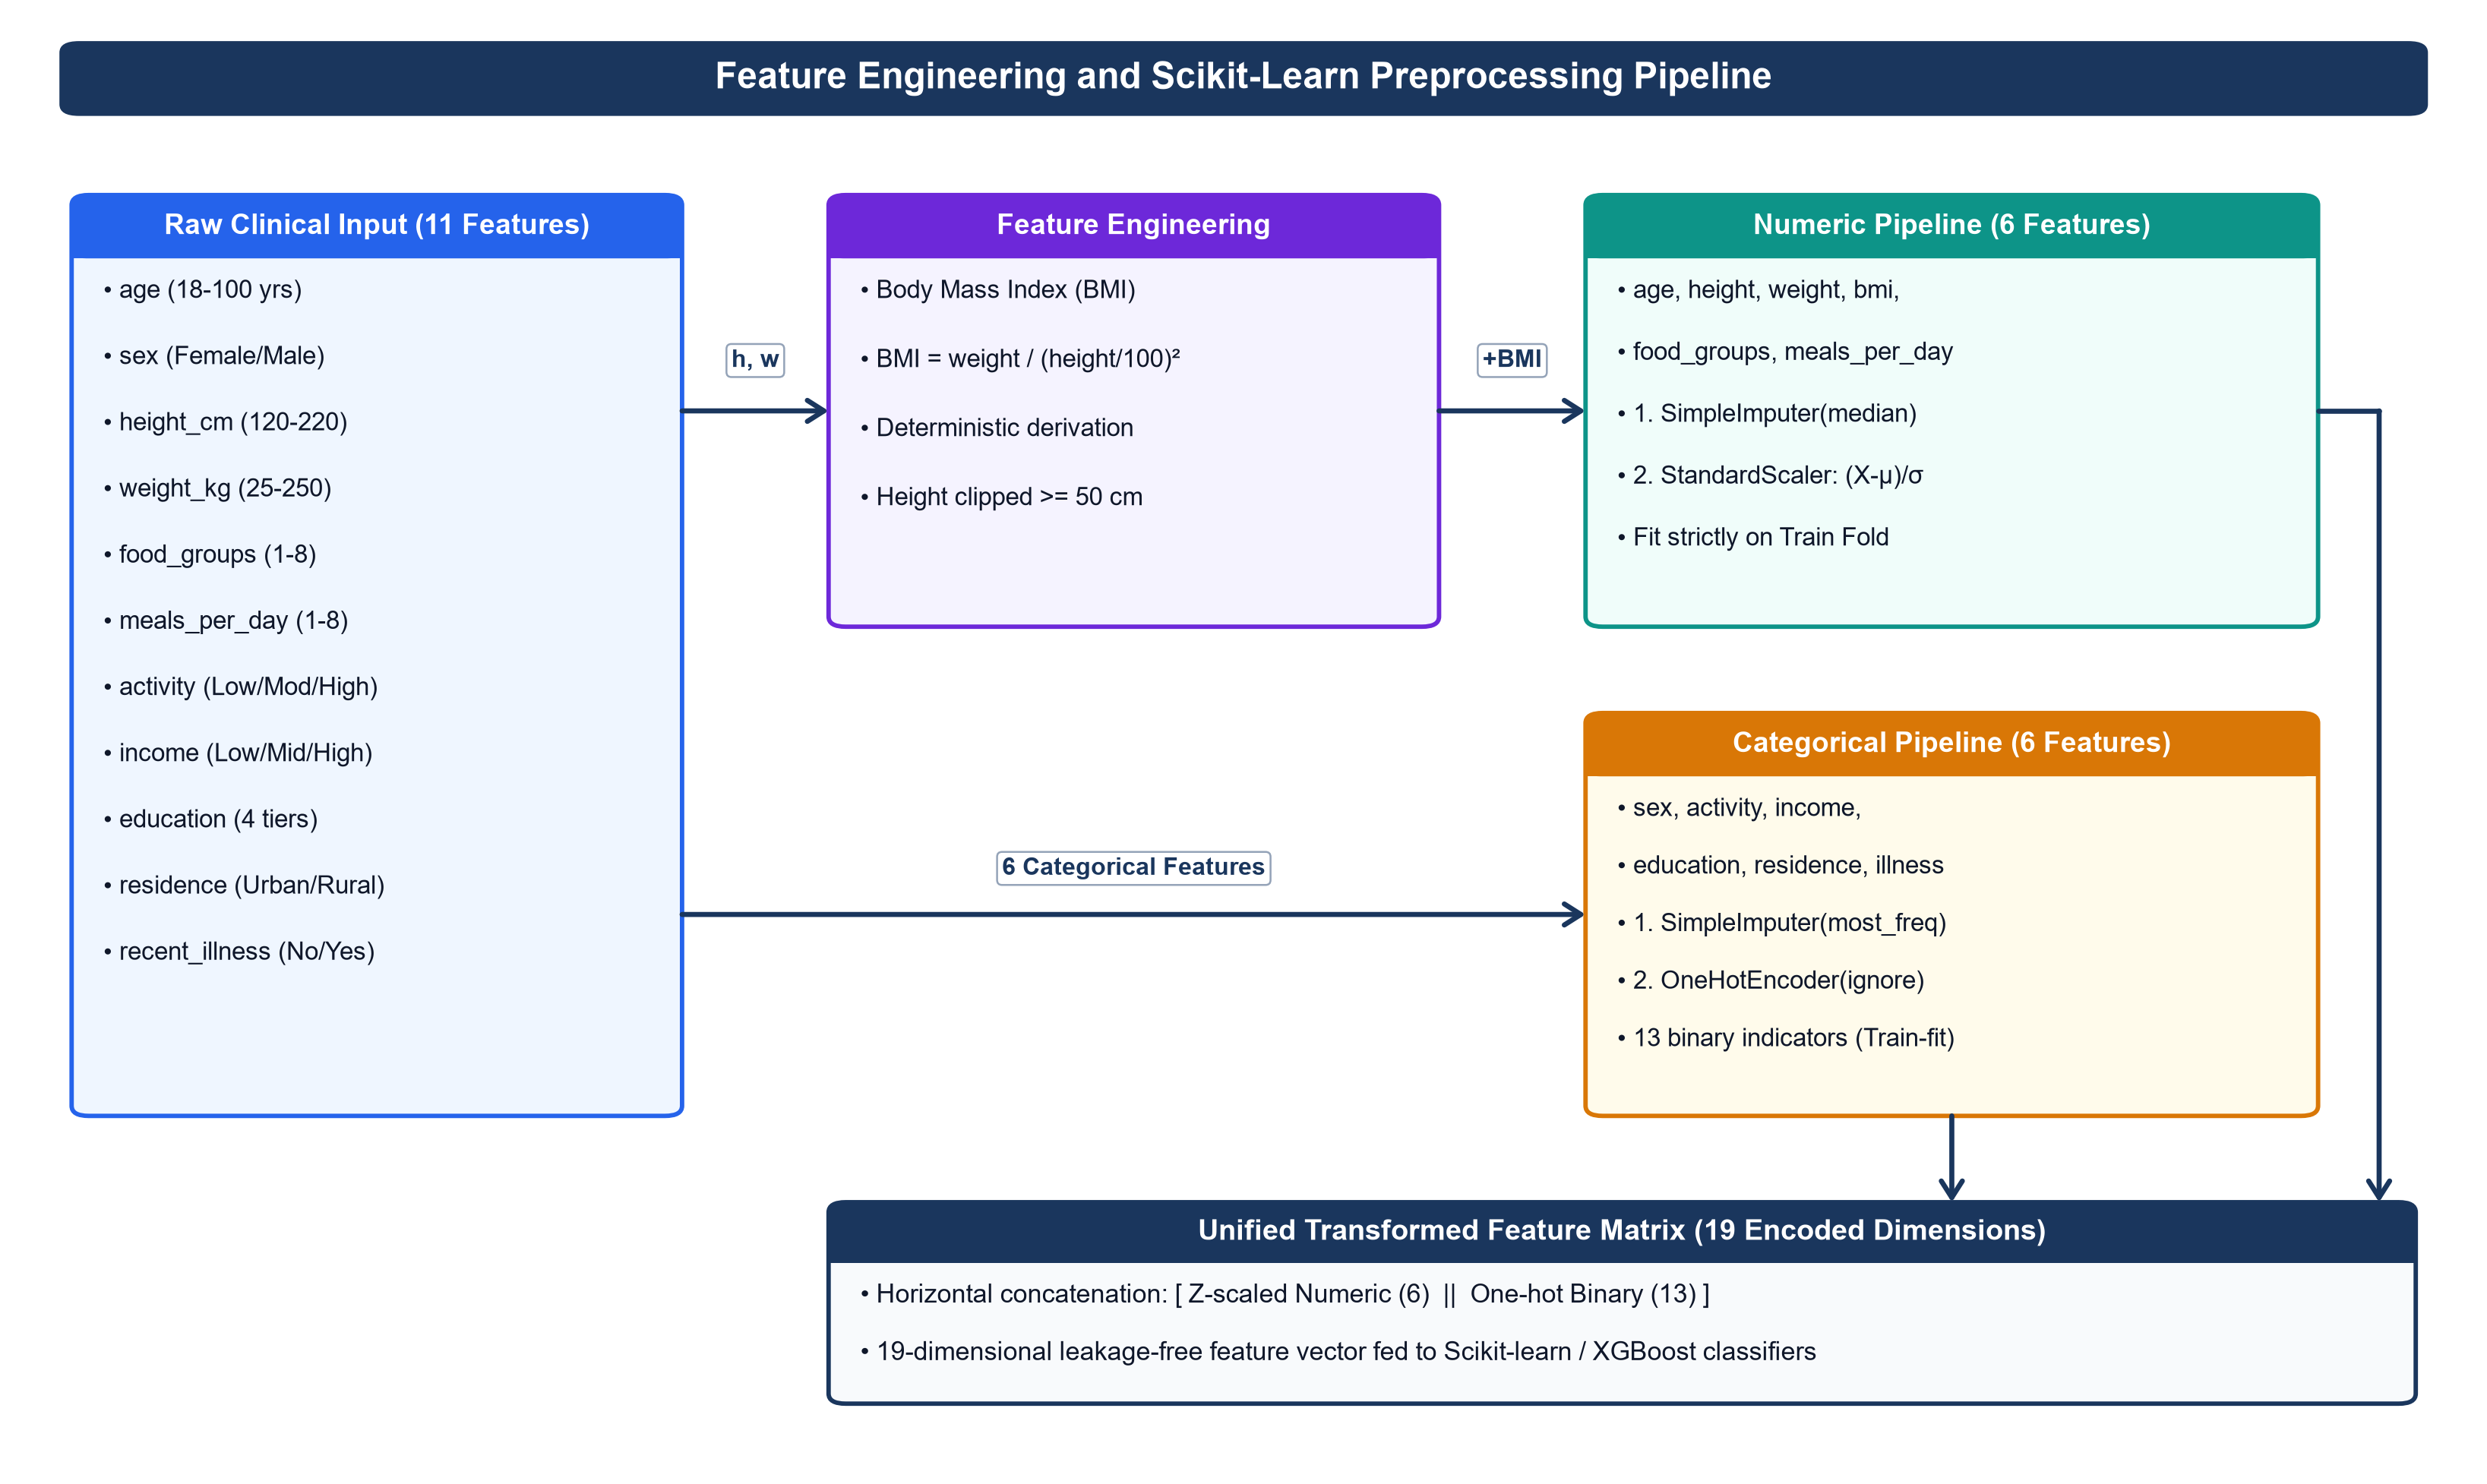
\includegraphics[width=0.95\textwidth]{figures/fig03_preprocessing_pipeline.png}
\caption{Feature engineering and leakage-free Scikit-learn preprocessing pipeline}
\label{fig:preproc_ch4}
\end{figure}

\section{Results \& Discussion}
Schema validation confirmed zero missing or out-of-range values across all $6{,}000$ records: \textbf{High Risk} ($2{,}195$, $36.58\%$), \textbf{Moderate Risk} ($2{,}103$, $35.05\%$), and \textbf{Low Risk} ($1{,}702$, $28.37\%$). Because labels originate from a calibrated scoring rule, this dataset serves as a reproducible software-testing and benchmarking cohort rather than standalone clinical proof.

% ------------------------------------------------------------------------------
% CHAPTER 5: OBJECTIVE 2 --- ML MODEL DEVELOPMENT \& BENCHMARKING
% ------------------------------------------------------------------------------
\chapter{Machine Learning Model Development \& Benchmarking}

\section{Introduction}
Building on Chapter 4's 19-dimensional leakage-free pipeline, Objective 2 benchmarks five supervised classifiers in \texttt{nutririsk/ml/training.py} to identify the optimal model for preliminary three-tier nutritional risk stratification.

\section{Problem Statement}
Linear classifiers often underfit non-linear multi-variable nutritional interactions (such as poor diet combined with advanced age and acute illness), whereas unconstrained trees risk overfitting. A rigorous cross-validation and holdout evaluation protocol is required.

\section{Methodology}
The $6{,}000$ records were partitioned via an 80:20 stratified split ($\text{random\_state} = 42$) into $4{,}800$ training and $1{,}200$ untouched holdout test records. Five-fold stratified CV was run inside the training set ($3{,}840$ train / $960$ validation per fold) across five candidate algorithms (Figure~\ref{fig:train_ch5}):
\begin{enumerate}
    \item \textbf{Logistic Regression:} Multinomial Softmax, L-BFGS, $C=1.0$, balanced weights.
    \item \textbf{Decision Tree (CART):} Gini impurity, $\text{max\_depth}=8$, balanced weights.
    \item \textbf{Random Forest:} $200$ trees, $\sqrt{D}$ split criterion, balanced weights.
    \item \textbf{Gradient Boosting:} $100$ sequential trees, deviance loss, $\eta = 0.1$.
    \item \textbf{XGBoost:} $250$ trees, $\text{max\_depth}=5$, $\eta=0.08$, subsample $0.9$, colsample\_bytree $0.9$, \texttt{mlogloss}.
\end{enumerate}

\begin{figure}[htbp]
\centering
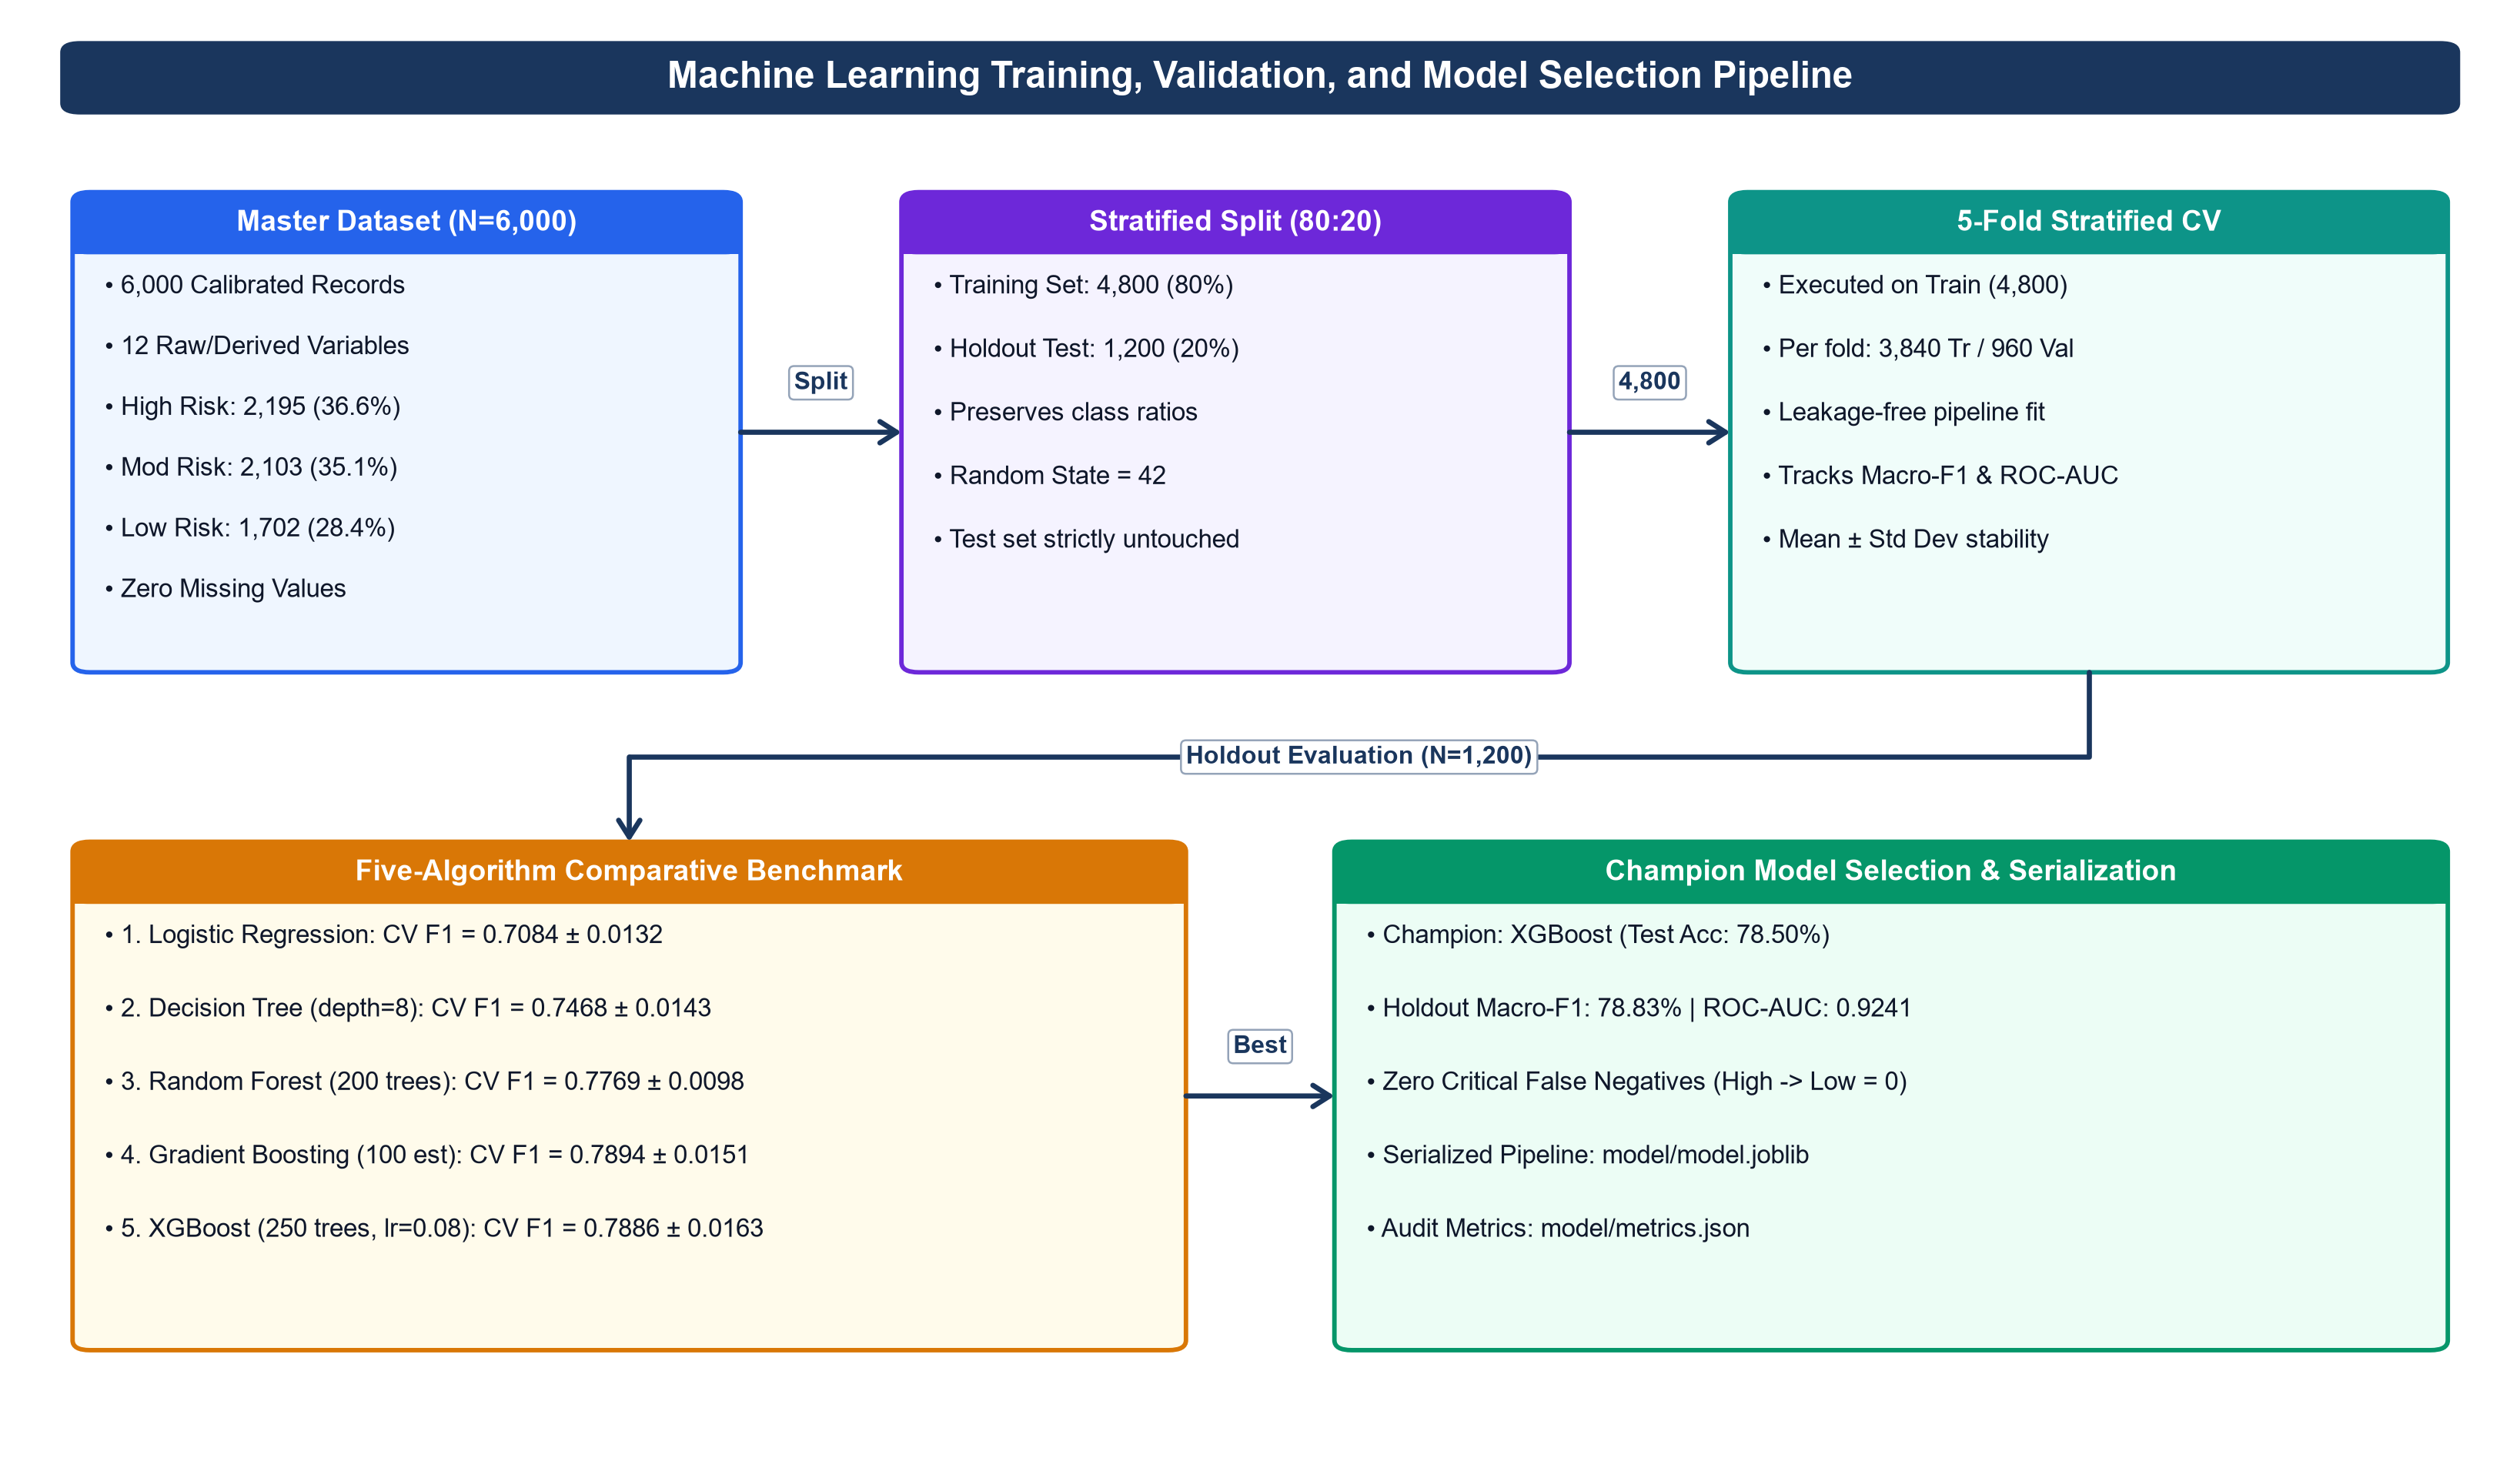
\includegraphics[width=0.95\textwidth]{figures/fig04_training_pipeline.png}
\caption{Machine learning training, 5-fold cross-validation, and model selection pipeline}
\label{fig:train_ch5}
\end{figure}

\section{Results \& Discussion}
As summarized in Table~\ref{tab:bench_ch5}, \textbf{XGBoost} outperformed all baselines on the unseen holdout set, achieving \textbf{78.50\%} accuracy, \textbf{79.10\%} Macro Precision, \textbf{78.61\%} Macro Recall, \textbf{78.83\%} Macro-F1, and \textbf{0.9241} OvR ROC-AUC, and was serialized to \texttt{model/model.joblib}.

\begin{table}[htbp]
\centering
\caption{Benchmark comparison of candidate ML models ($N_{\text{train}}=4{,}800$, $N_{\text{test}}=1{,}200$)}
\label{tab:bench_ch5}
\resizebox{\textwidth}{!}{%
\begin{tabular}{@{}lcccccc@{}}
\toprule
\textbf{Model} & \textbf{5-Fold CV F1} & \textbf{Accuracy} & \textbf{Macro Precision} & \textbf{Macro Recall} & \textbf{Macro-F1} & \textbf{ROC-AUC (OvR)} \\ \midrule
Logistic Regression & $0.7084 \pm 0.0132$ & 70.67\% & 70.87\% & 70.68\% & 70.77\% & 0.8711 \\
Decision Tree & $0.7468 \pm 0.0143$ & 74.17\% & 75.87\% & 74.15\% & 74.71\% & 0.8820 \\
Random Forest & $0.7769 \pm 0.0098$ & 76.67\% & 77.29\% & 76.60\% & 76.88\% & 0.9140 \\
Gradient Boosting & $\mathbf{0.7894 \pm 0.0151}$ & 77.75\% & 78.82\% & 77.60\% & 78.06\% & 0.9237 \\
\textbf{XGBoost (Champion)} & $0.7886 \pm 0.0163$ & \textbf{78.50\%} & \textbf{79.10\%} & \textbf{78.61\%} & \textbf{78.83\%} & \textbf{0.9241} \\ \bottomrule
\end{tabular}%
}
\end{table}

% ------------------------------------------------------------------------------
% CHAPTER 6: OBJECTIVE 3 --- DUAL EXPLAINABLE AI \& SAFETY VERIFICATION
% ------------------------------------------------------------------------------
\chapter{Dual Explainable AI (XAI) \& Triage Safety Verification}

\section{Introduction}
Objective 3 resolves the black-box barrier in clinical ML by pairing cooperative-game-theoretic \texttt{TreeSHAP} attributions with occlusion-based sensitivity analysis in \texttt{nutririsk/ml/explainability.py}, alongside asymmetric safety auditing against critical false negatives.

\section{Problem Statement}
Tree ensembles distribute decision logic across 250 boosted trees, and one-hot encoding splits categorical attributes across multiple binary columns. Clinicians require aggregated, indicator-level explanations and assurance that High-Risk patients are never misclassified as Low Risk.

\section{Methodology}
\begin{enumerate}
    \item \textbf{TreeSHAP Attributions:} \texttt{shap.TreeExplainer} \cite{lundberg2017unified} computes exact Shapley values $\phi_j$ in margin space and aggregates one-hot columns back to each clinical indicator group.
    \item \textbf{Occlusion Sensitivity:} Each feature group is masked with its population median/mode to quantify probability shift $\Delta P_c = P(c \mid \mathbf{x}) - P(c \mid \mathbf{x}_{\text{masked}})$ (Figure~\ref{fig:xai_ch6}).
    \item \textbf{Asymmetric Safety Criterion:} On the confusion matrix $\mathbf{C}$, we enforce $\text{FN}_{\text{critical}} = \mathbf{C}_{2,0} = 0$ (High Risk predicted as Low Risk).
\end{enumerate}

\begin{figure}[htbp]
\centering
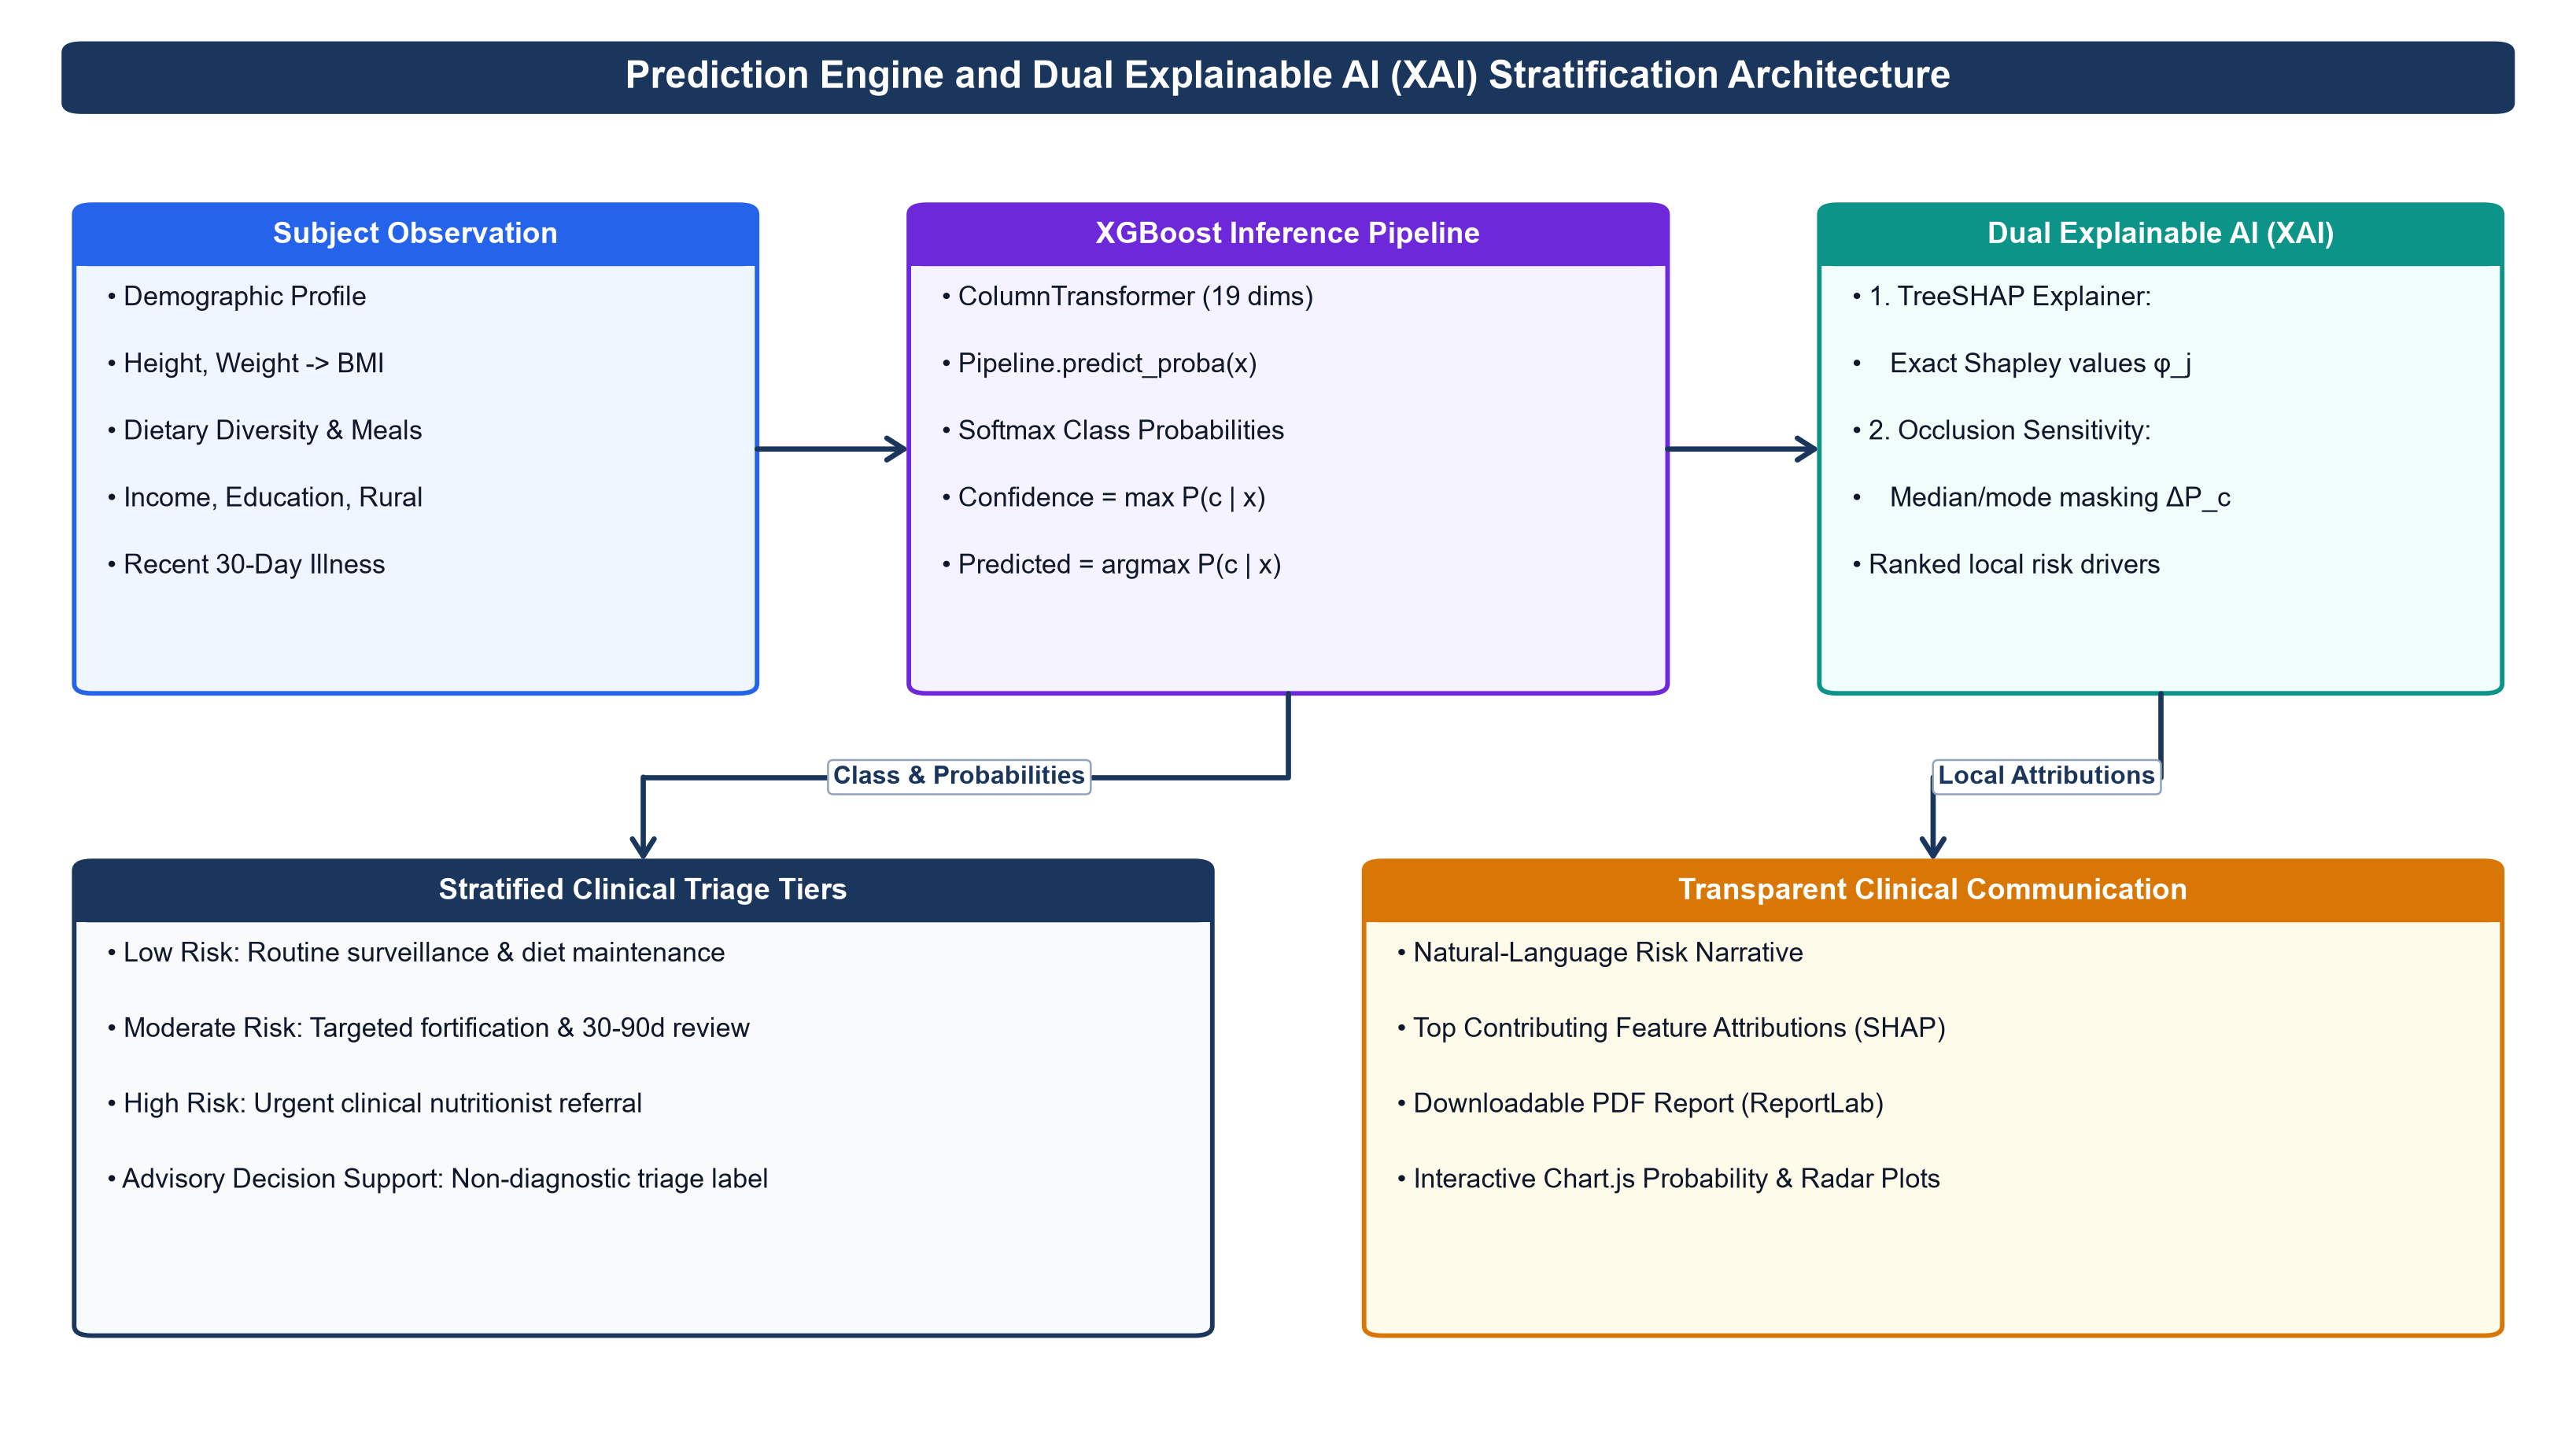
\includegraphics[width=0.95\textwidth]{figures/fig05_prediction_stratification.png}
\caption{Prediction inference and Dual Explainable AI (XAI) stratification workflow}
\label{fig:xai_ch6}
\end{figure}

\section{Results \& Discussion}
Table~\ref{tab:perm_ch6} confirms that XGBoost relies on biologically and socioeconomically meaningful indicators---Dietary Diversity ($0.1739$), Chronological Age ($0.1645$), Recent Illness ($0.1072$), and BMI ($0.0906$)---while assigning negligible weight to biological sex ($0.0000$). These attributions represent predictive model associations rather than direct causal effects.

\begin{table}[htbp]
\centering
\caption{Global permutation feature importance rankings for XGBoost champion}
\label{tab:perm_ch6}
\resizebox{\textwidth}{!}{%
\begin{tabular}{@{}clcc@{}}
\toprule
\textbf{Rank} & \textbf{Clinical / Demographic Indicator} & \textbf{Mean Importance} & \textbf{Relative Share} \\ \midrule
1 & Dietary Diversity (\texttt{food\_groups}) & \textbf{0.1739} & 24.71\% \\
2 & Chronological Age (\texttt{age}) & \textbf{0.1645} & 23.37\% \\
3 & Recent Febrile/Diarrheal Illness (\texttt{recent\_illness}) & \textbf{0.1072} & 15.23\% \\
4 & BMI (Height \& Weight) & \textbf{0.0906} & 12.87\% \\
5 & Household Income (\texttt{income}) & 0.0773 & 10.98\% \\
6 & Meal Frequency (\texttt{meals\_per\_day}) & 0.0655 & 9.31\% \\
7 & Residence Environment (\texttt{residence}) & 0.0217 & 3.08\% \\
8 & Physical Activity (\texttt{activity}) & 0.0095 & 1.35\% \\
9 & Biological Sex (\texttt{sex}) & 0.0000 & 0.00\% \\
10 & Education Level (\texttt{education}) & -0.0006 & -0.09\% \\ \bottomrule
\end{tabular}%
}
\end{table}

% ------------------------------------------------------------------------------
% CHAPTER 7: SYSTEM DESIGN, IMPLEMENTATION \& METHODOLOGY
% ------------------------------------------------------------------------------
\chapter{System Design, Implementation \& Methodology}

\section{Proposed Architecture}
Figure~\ref{fig:arch_ch7} presents the four-tier modular architecture of NutriRisk AI: Tier 1 Presentation (HTML5, Bootstrap 5, Chart.js), Tier 2 Application Controller \& Security (Flask 3.1.3 Blueprints, Scrypt, OTP, CSRF, ReportLab), Tier 3 ML \& XAI Engine (ColumnTransformer, XGBoost, TreeSHAP), and Tier 4 Persistence (SQLite \& Joblib).

\begin{figure}[htbp]
\centering
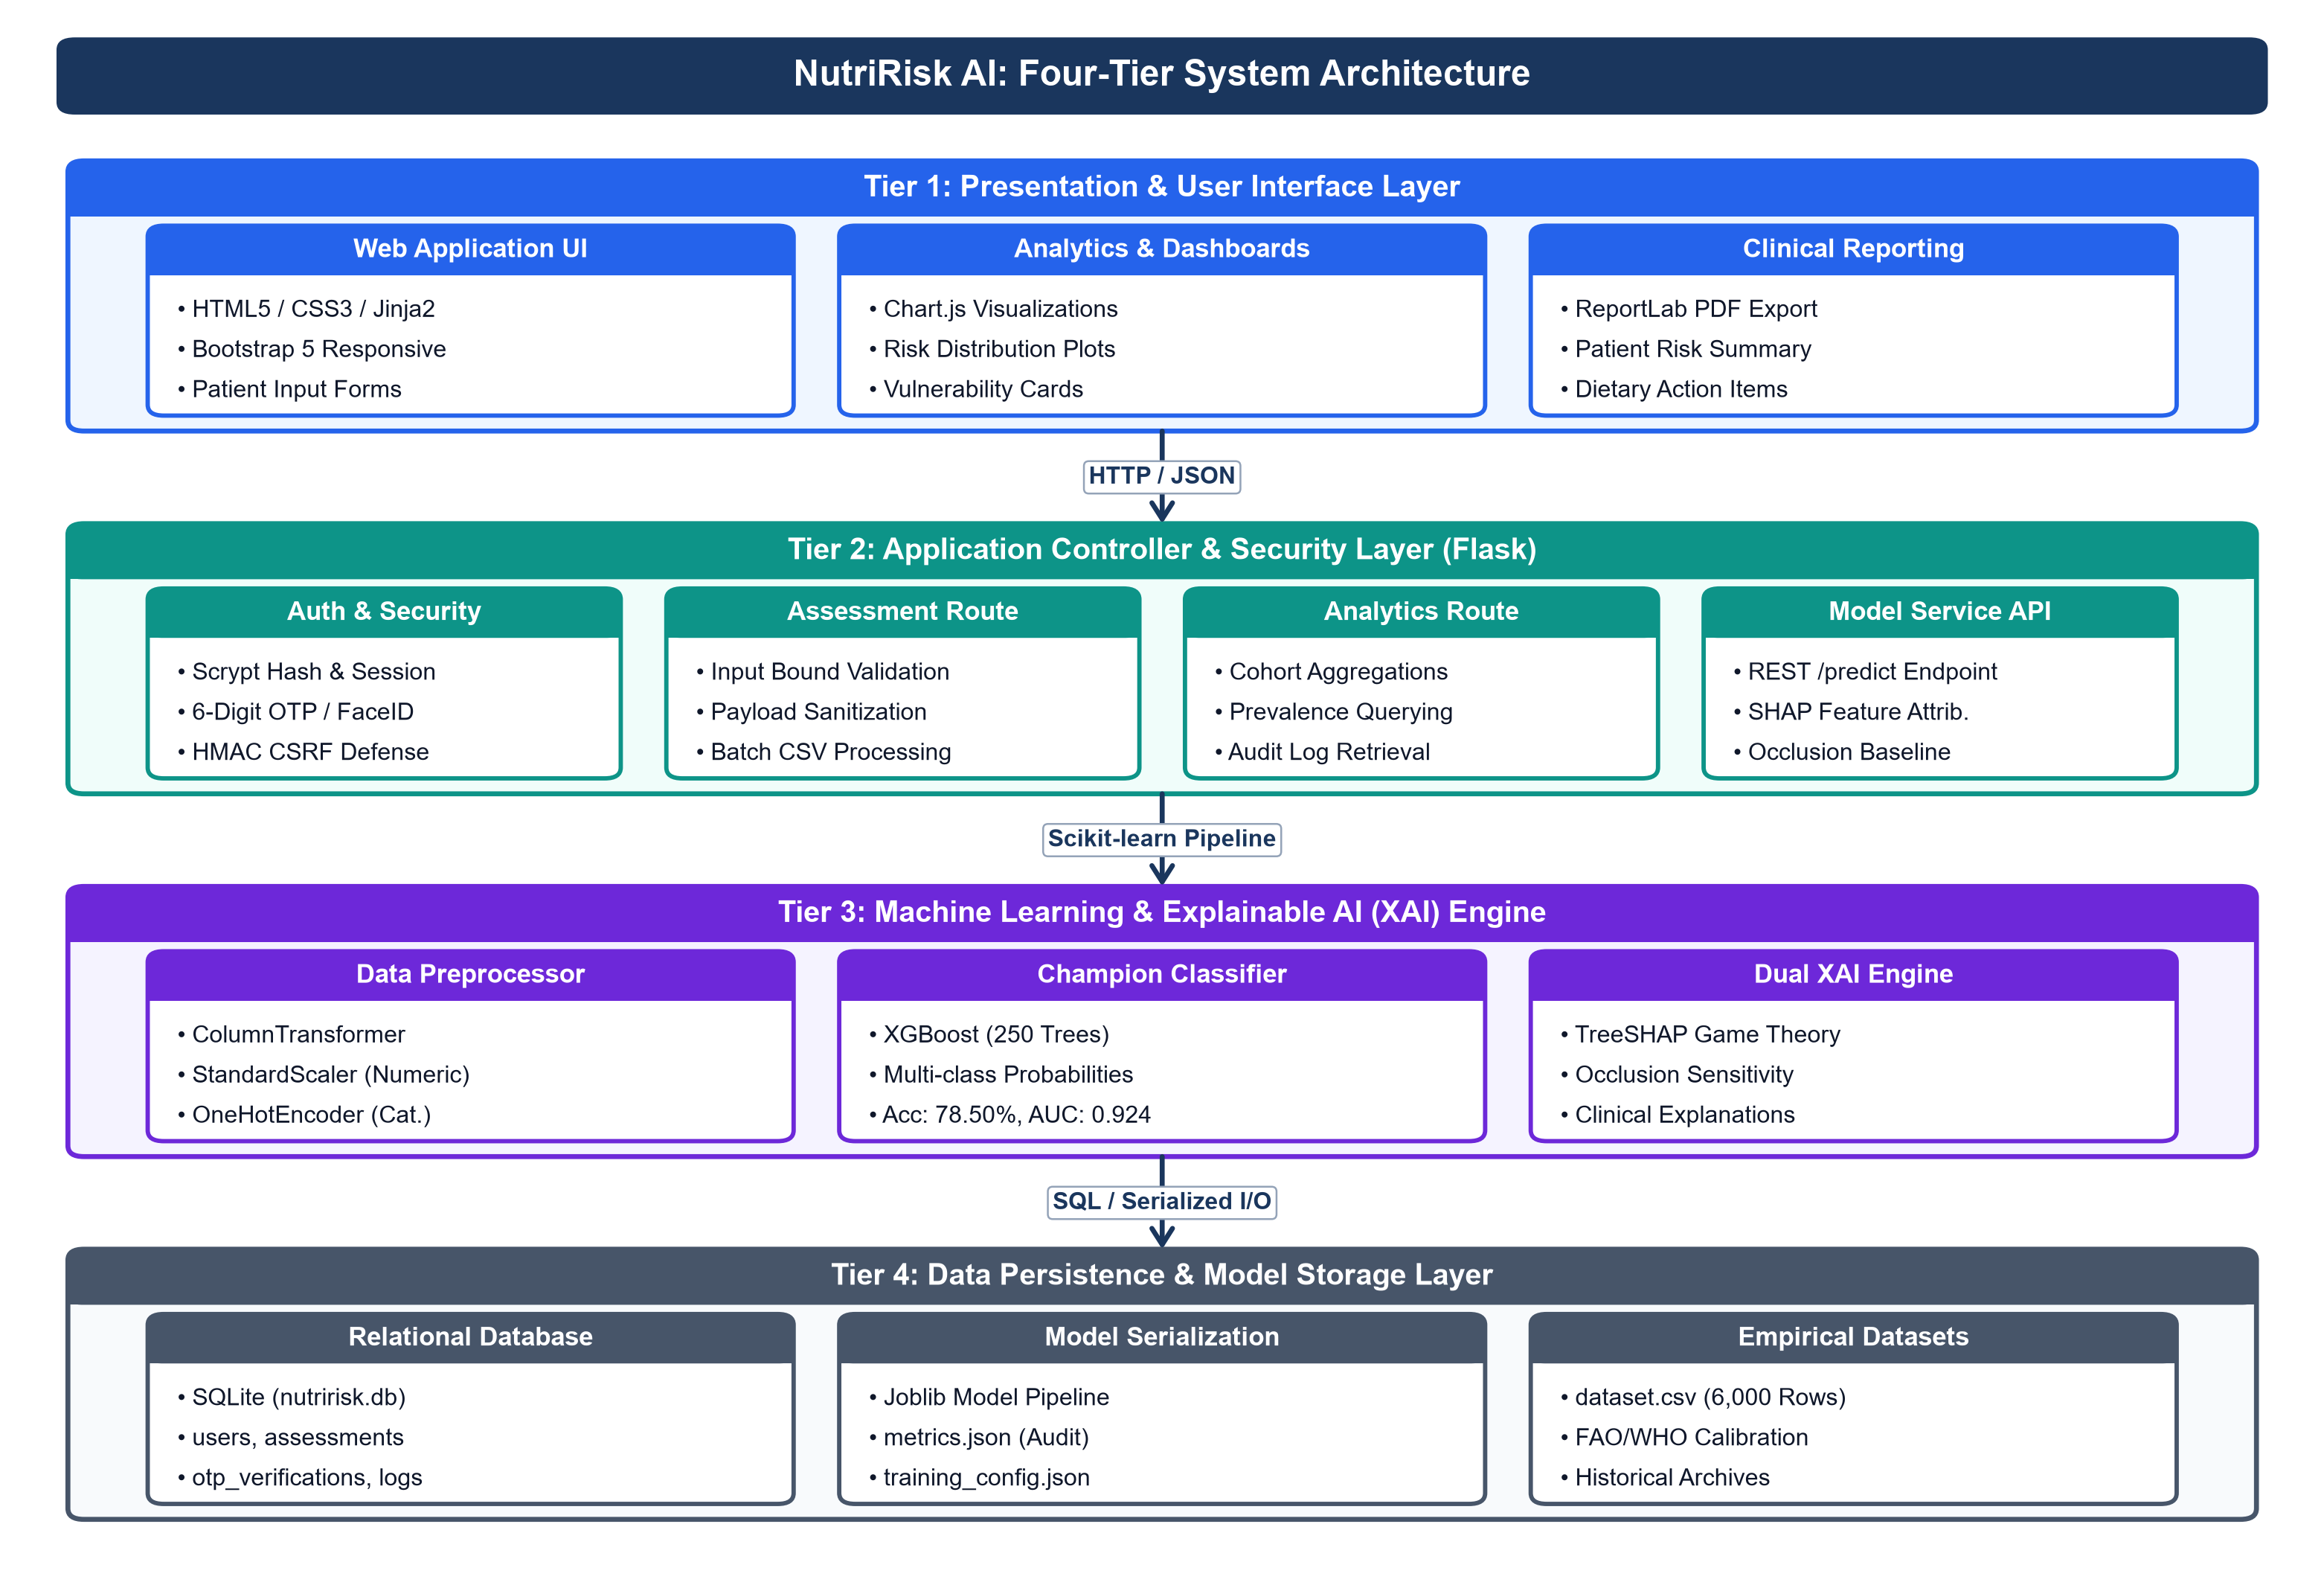
\includegraphics[width=0.95\textwidth]{figures/fig01_system_architecture.png}
\caption{Four-tier system architecture of NutriRisk AI}
\label{fig:arch_ch7}
\end{figure}

\section{Data Flow and Operational Workflow}
Figure~\ref{fig:workflow_ch7} depicts the end-to-end data flow from raw demographic/dietary capture through range validation, preprocessing, XGBoost inference, dual XAI attribution, and three-tier stratification.

\begin{figure}[htbp]
\centering
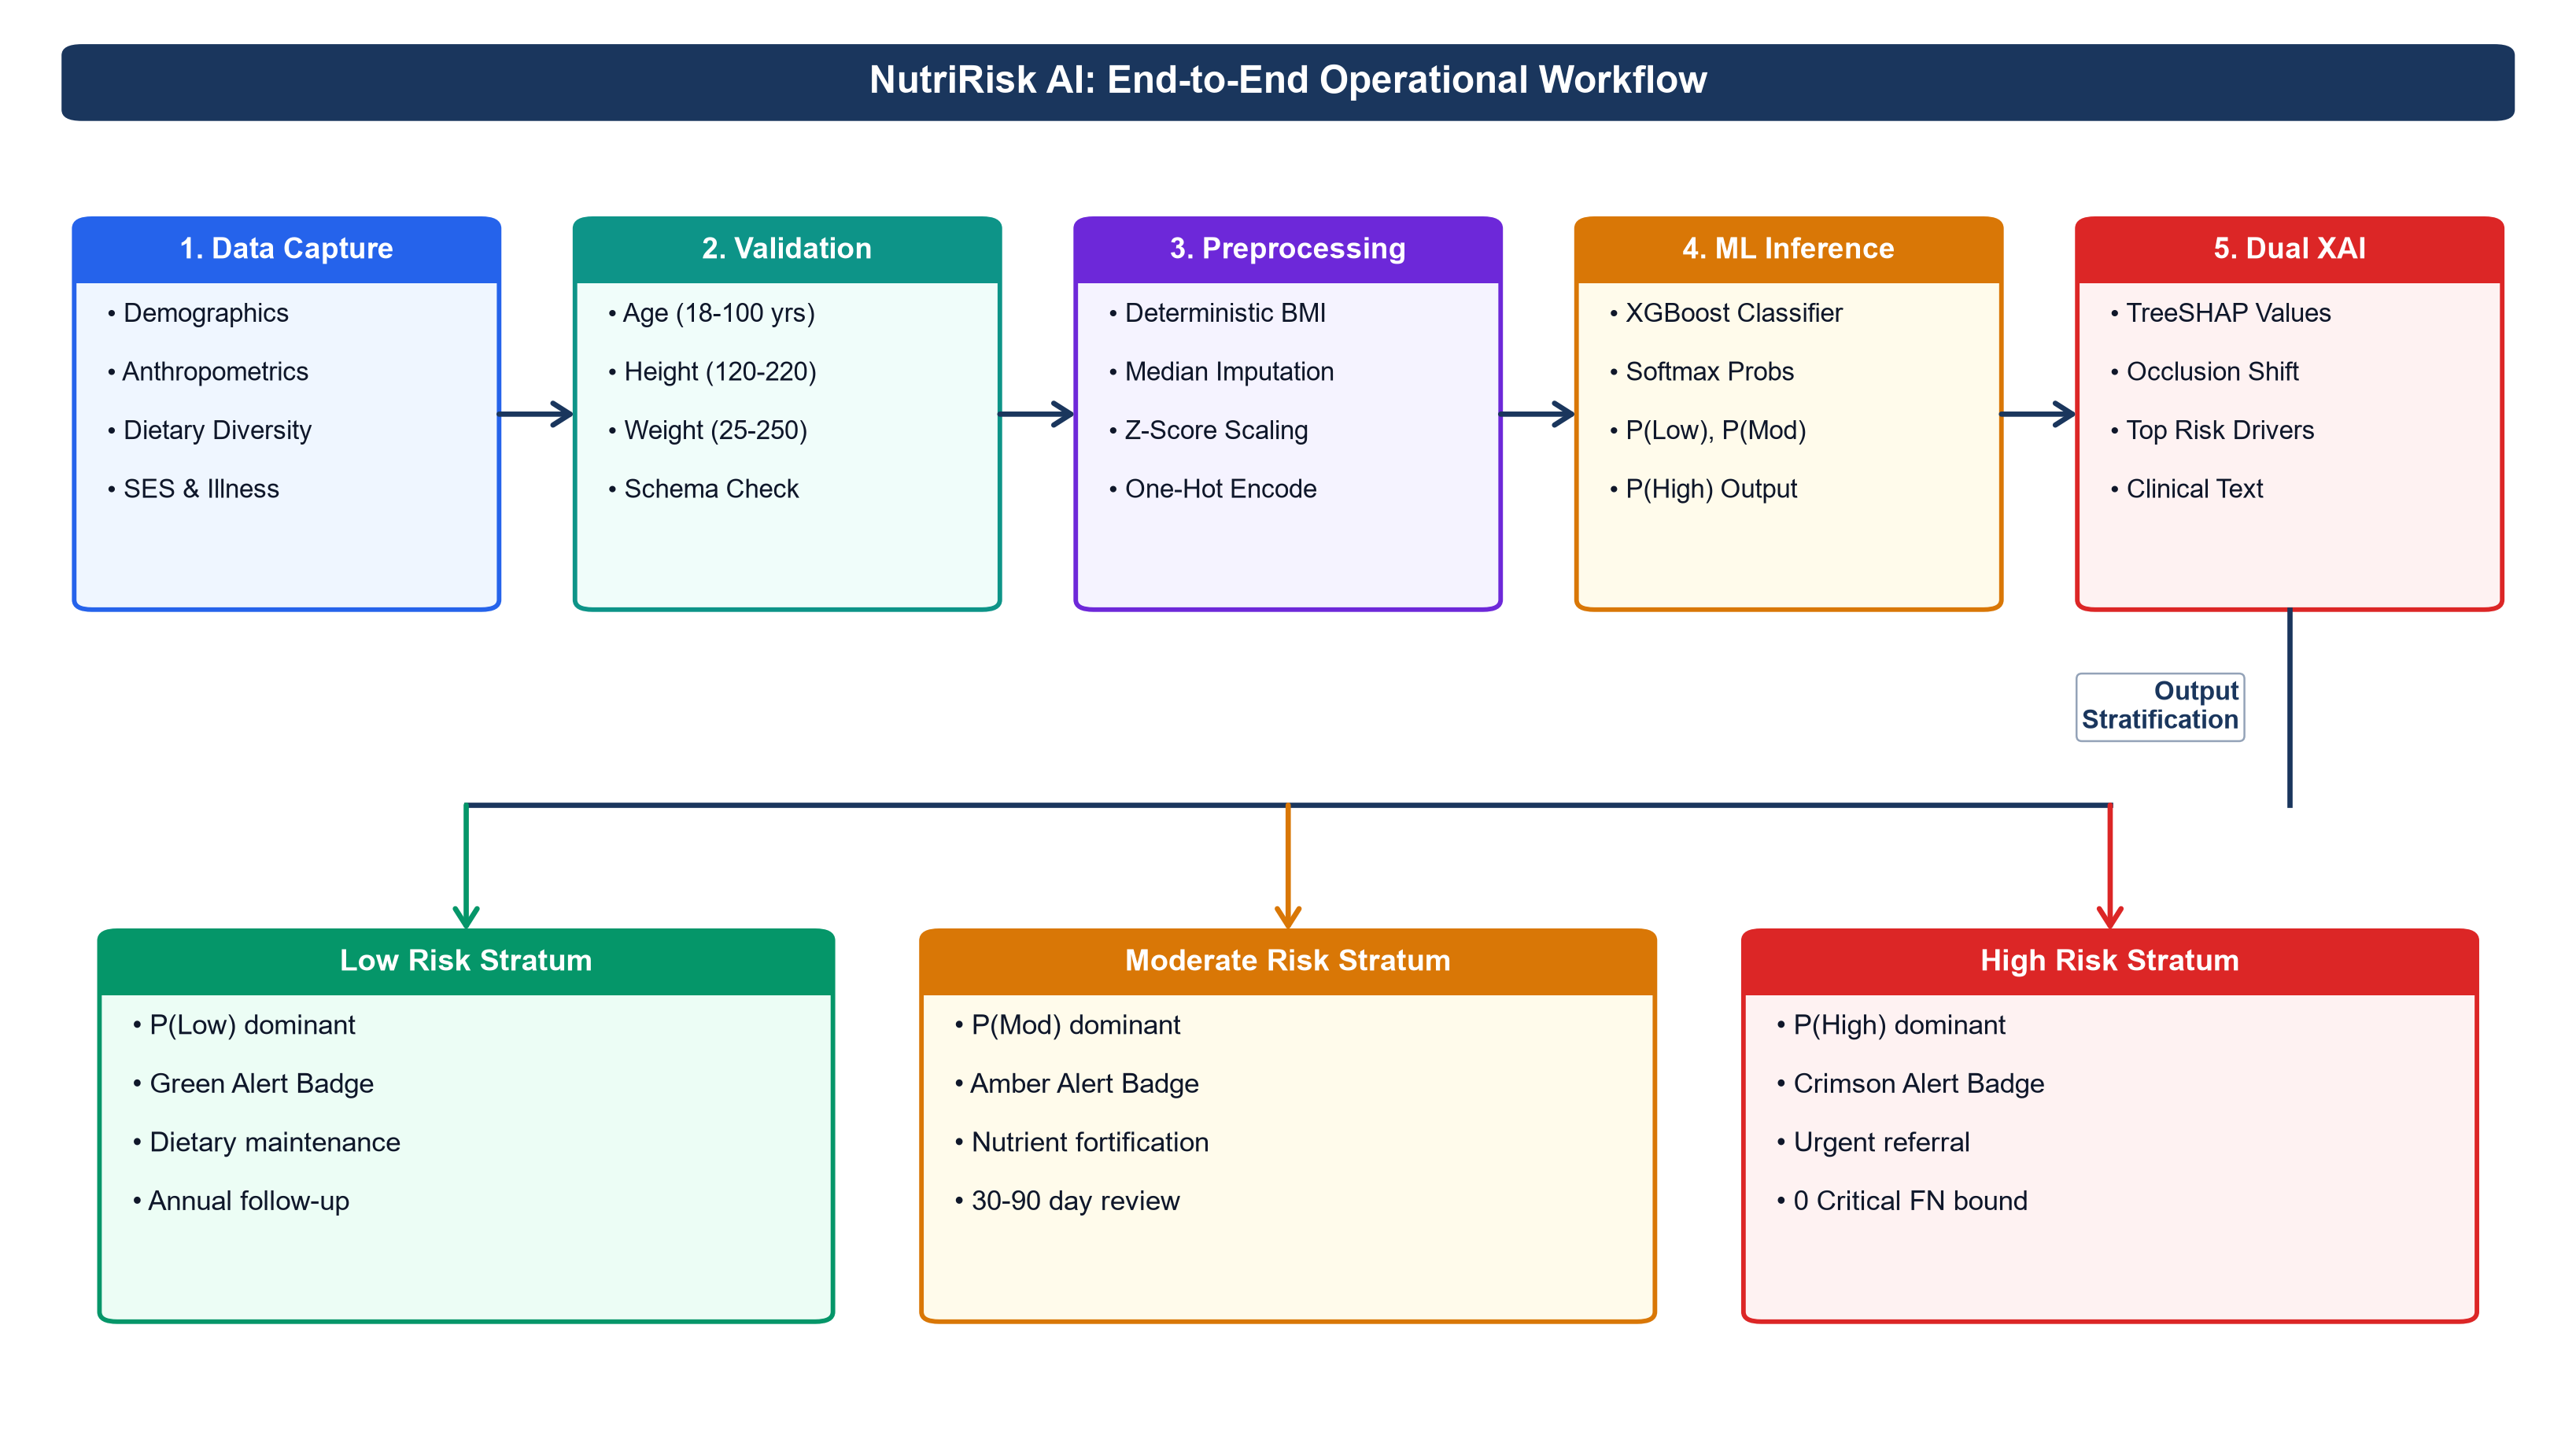
\includegraphics[width=0.95\textwidth]{figures/fig02_nutririsk_workflow.png}
\caption{End-to-end operational workflow of NutriRisk AI}
\label{fig:workflow_ch7}
\end{figure}

\section{UML, Database ER, and Sequence Diagrams}
Figure~\ref{fig:er_ch7} shows the five-table SQLite Entity-Relationship schema (\texttt{users}, \texttt{assessments}, \texttt{otp\_verifications}, \texttt{admin\_audit\_logs}, \texttt{model\_metadata}), and Figure~\ref{fig:seq_ch7} illustrates the runtime interaction sequence from user submission to CSRF verification, ML/XAI execution, SQLite commit, and PDF export.

\begin{figure}[htbp]
\centering
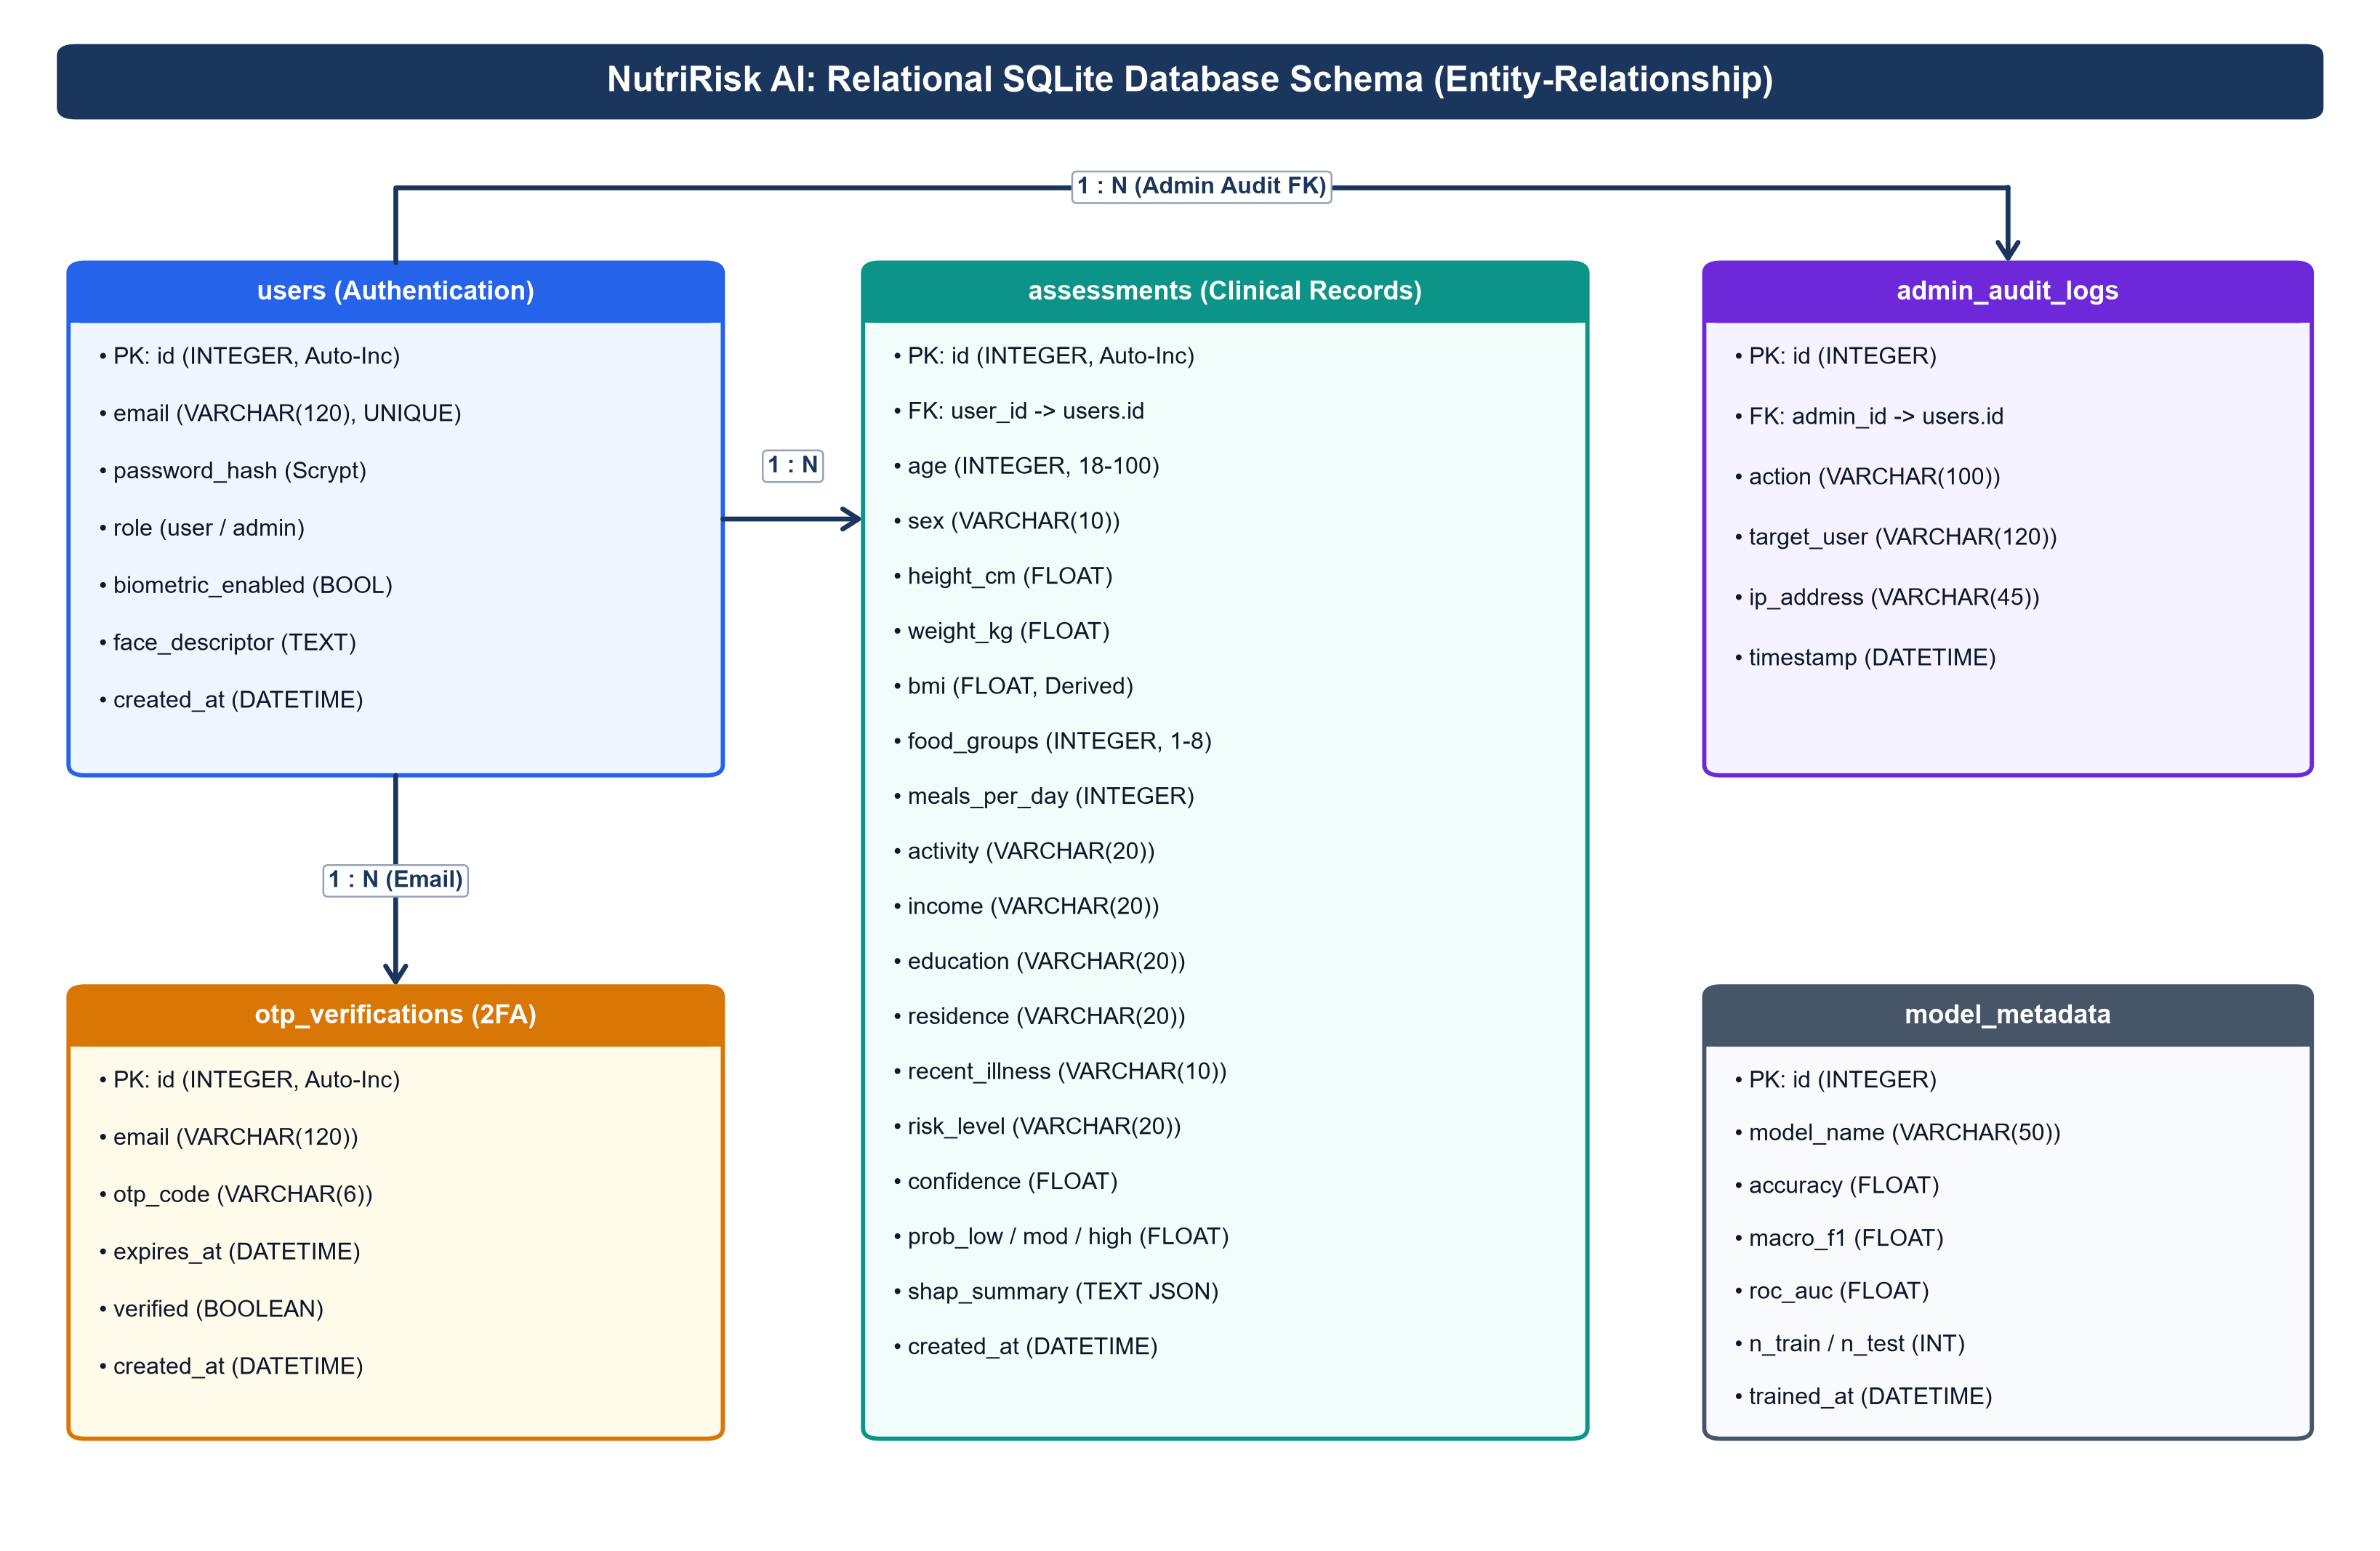
\includegraphics[width=0.92\textwidth]{figures/fig06_database_er.png}
\caption{Relational SQLite database Entity-Relationship (ER) schema}
\label{fig:er_ch7}
\end{figure}

\begin{figure}[htbp]
\centering
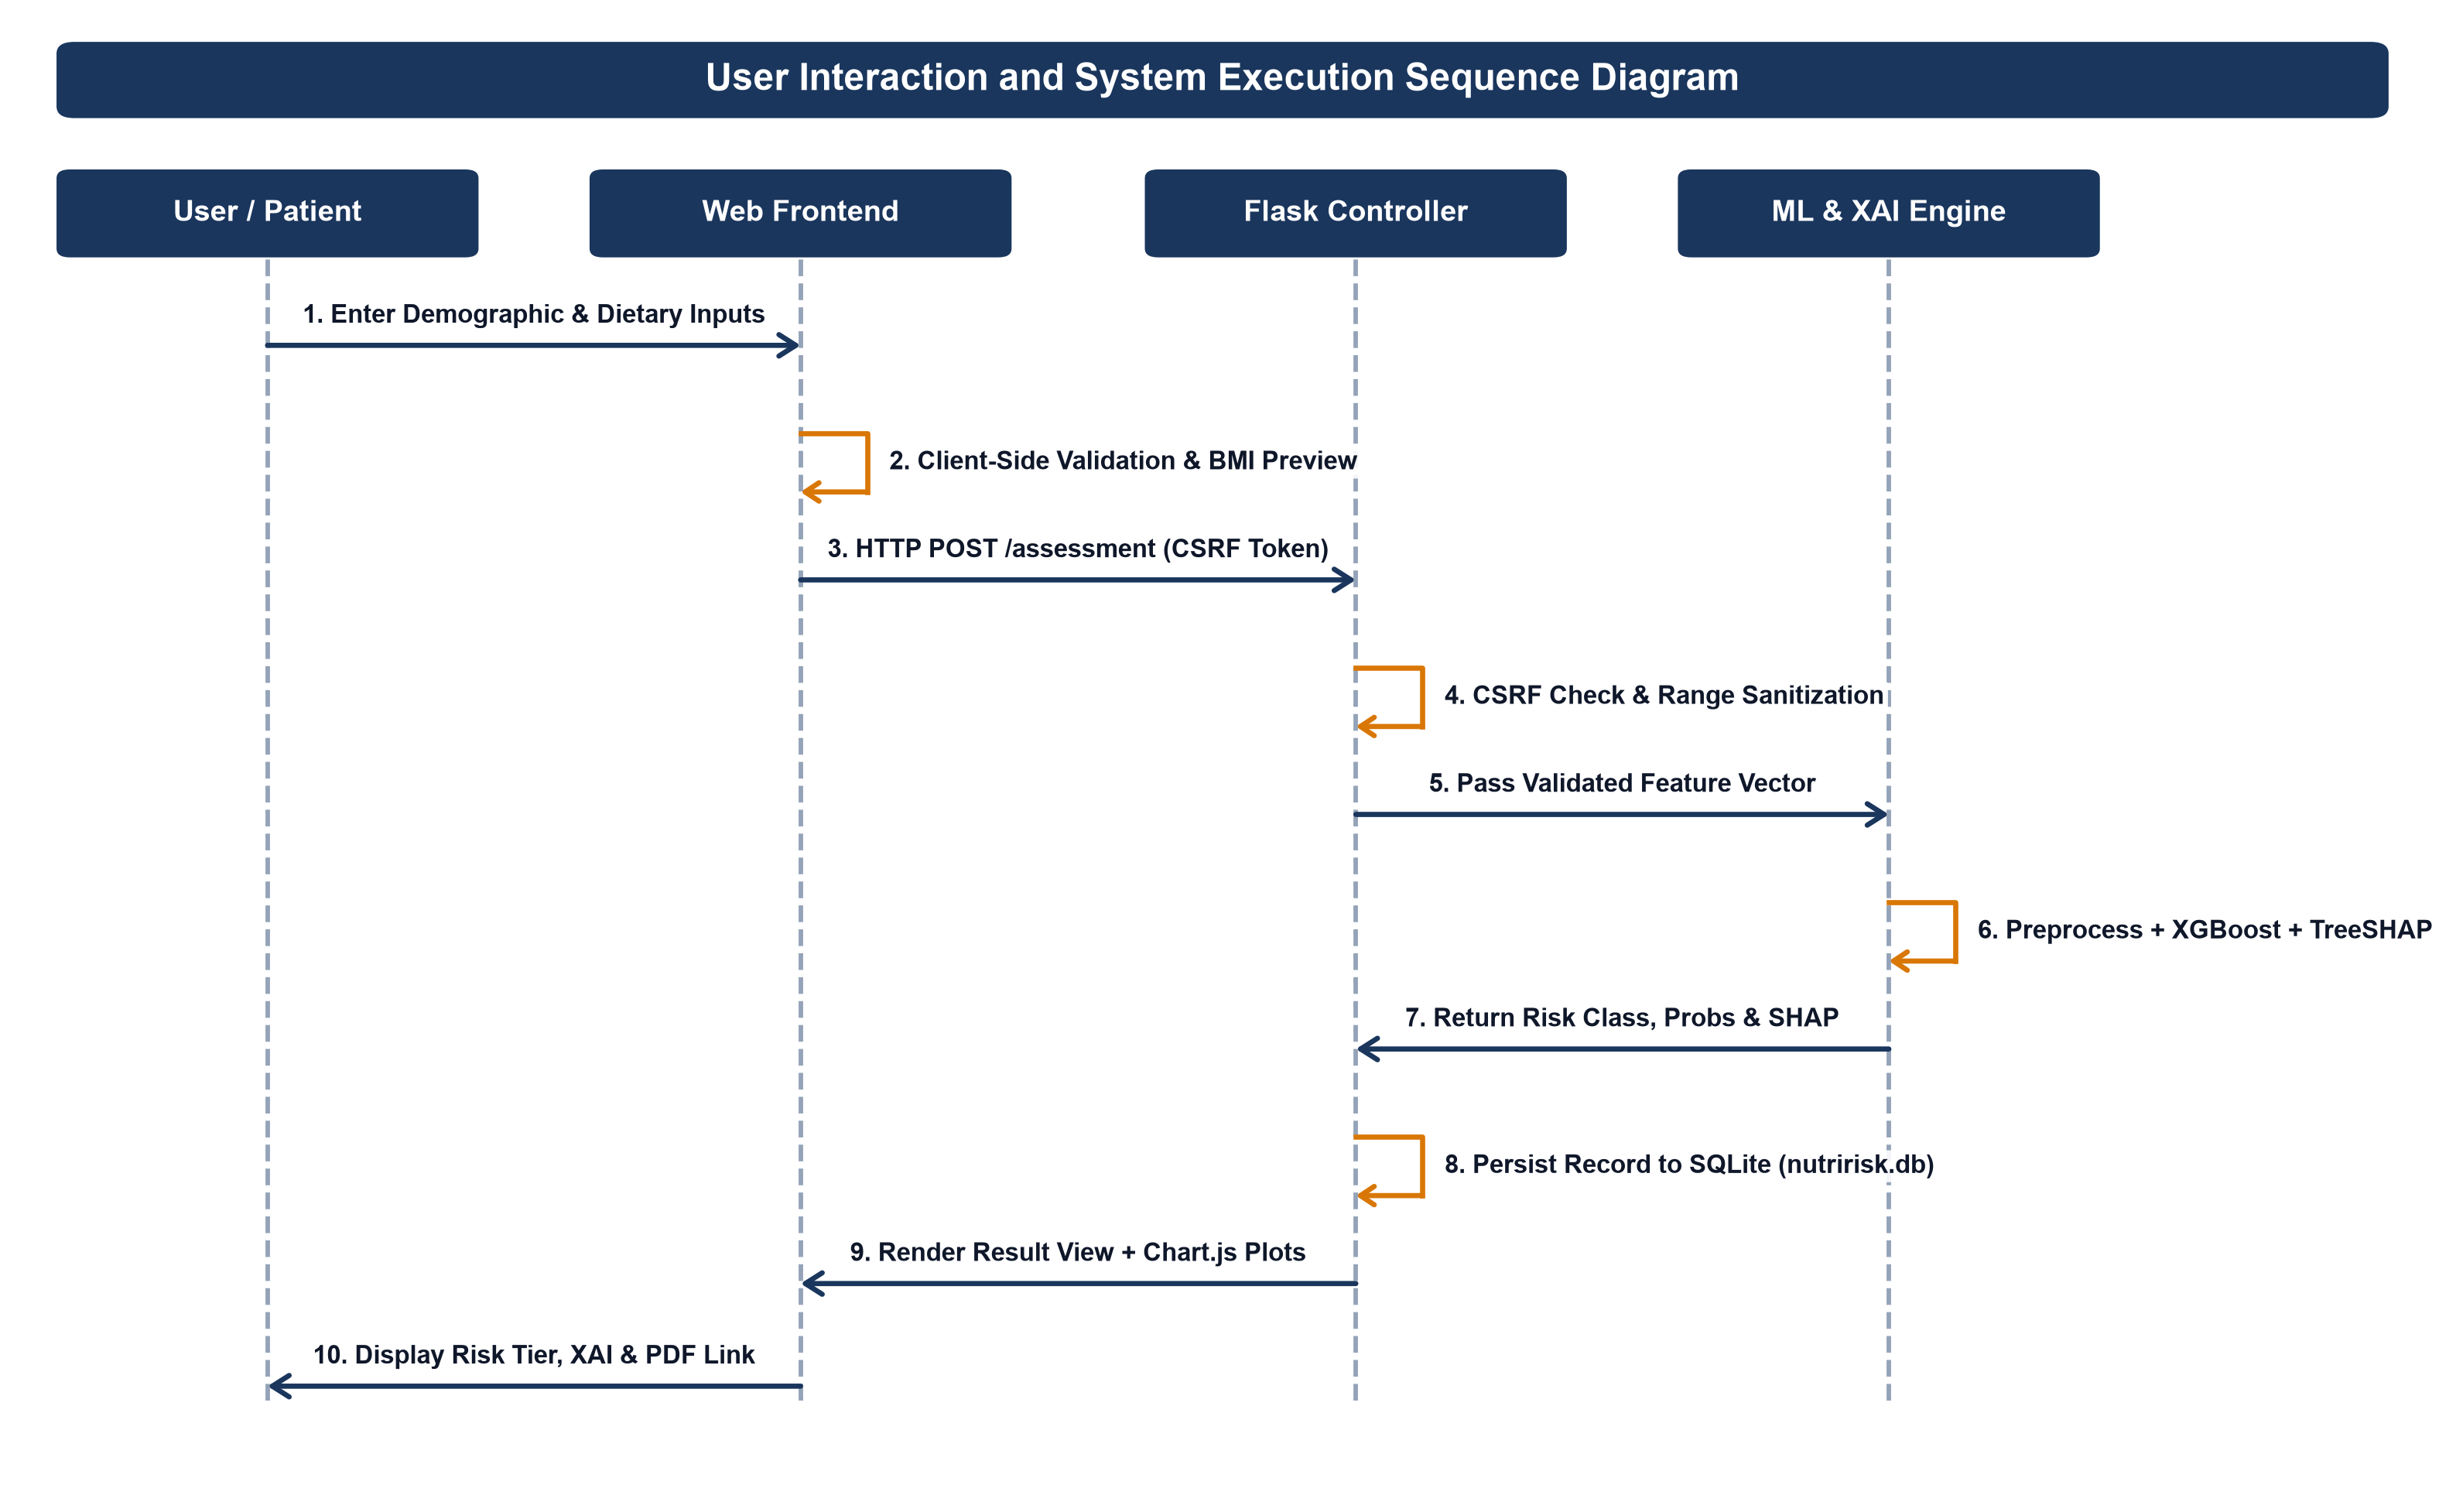
\includegraphics[width=0.92\textwidth]{figures/fig07_user_interaction.png}
\caption{User interaction and system execution sequence diagram}
\label{fig:seq_ch7}
\end{figure}

\section{Dataset Description}
The Phase-I cohort (\texttt{data/dataset.csv}) contains $N = 6{,}000$ adult records ($18$--$90$ years) across 3 classes (High: $2{,}195$, Moderate: $2{,}103$, Low: $1{,}702$) with zero missing values.

\section{Data Pre-processing}
Median imputation + \texttt{StandardScaler} for 6 numeric features and mode imputation + \texttt{OneHotEncoder} for 6 categorical features, fitted strictly on the $4{,}800$-record training split.

\section{Feature Engineering}
Deterministic derivation of Body Mass Index ($\text{BMI} = \text{weight\_kg} / (\text{height\_cm}/100)^2$) with height clipped $\ge 50$ cm, expanding 11 raw inputs into 12 base features and 19 encoded dimensions.

\section{Algorithm Selection}
XGBoost ($250$ estimators, $\text{max\_depth}=5$, $\eta=0.08$, subsample $0.9$, colsample\_bytree $0.9$) was selected as the champion classifier over Logistic Regression, Decision Tree, Random Forest, and Gradient Boosting based on highest holdout accuracy ($78.50\%$), Macro-F1 ($78.83\%$), ROC-AUC ($0.9241$), and zero critical false negatives.

\section{Model Training}
Training minimizes regularized multiclass cross-entropy loss (\texttt{mlogloss}) with 5-fold stratified CV on the $4{,}800$ training samples before final evaluation on the $1{,}200$ holdout test samples.

\section{Web Application Implementation and Live Screens}
The Flask 3.1.3 application is structured across modular Blueprints (\texttt{auth}, \texttt{main}, \texttt{assessment}, \texttt{analytics}, \texttt{admin}) and 16 Jinja2 templates. Figures~\ref{fig:ss01}--\ref{fig:ss10} present live screenshots captured from the running NutriRisk AI application.

\begin{figure}[htbp]
\centering
\begin{minipage}[b]{0.48\textwidth}
    \centering
    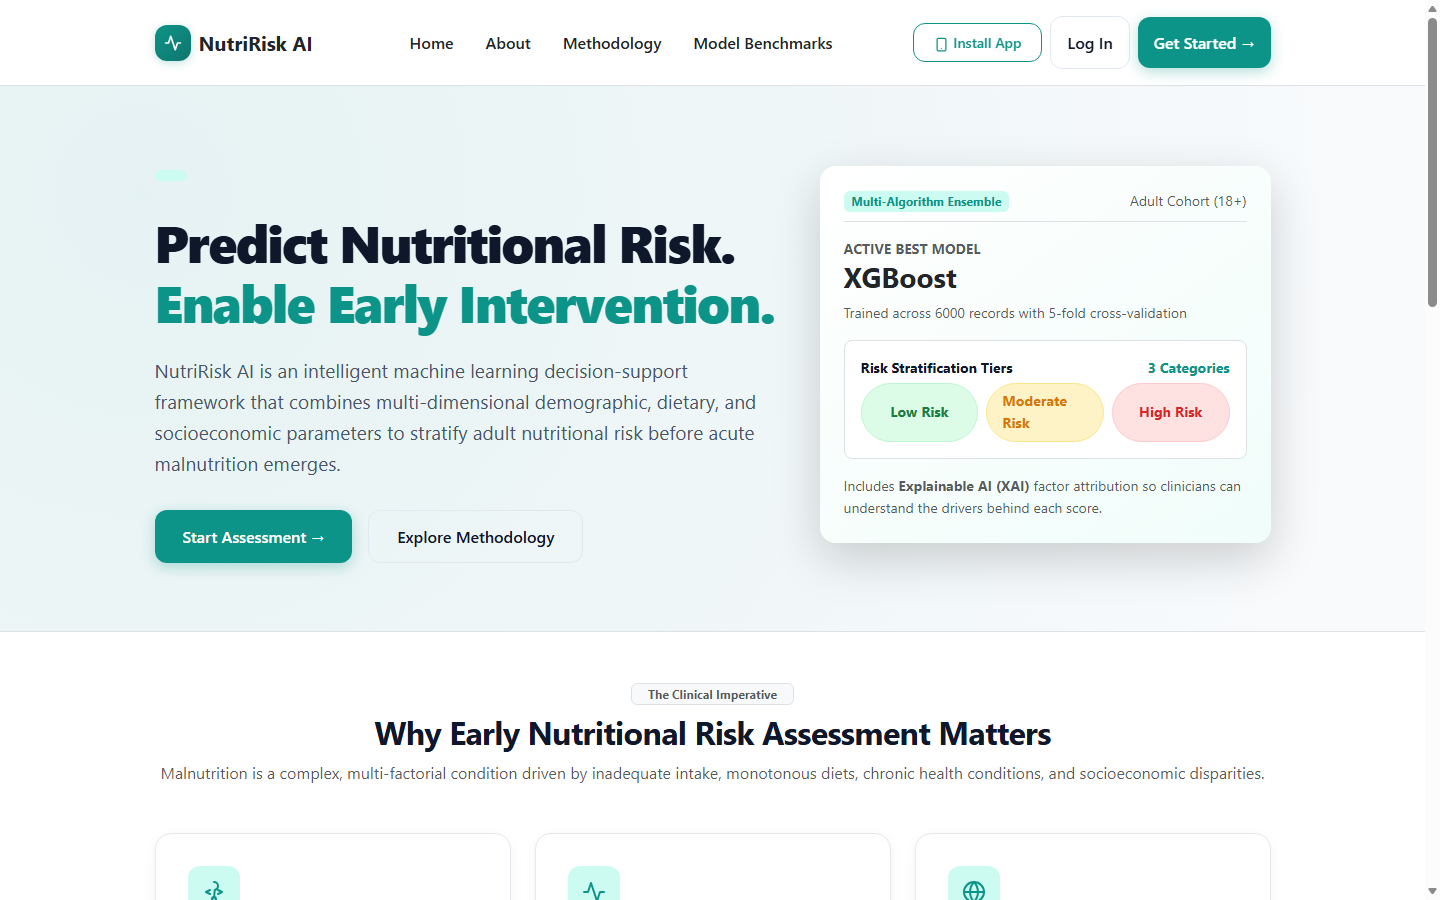
\includegraphics[width=\textwidth]{screenshots/ss01_welcome.png}
    \caption{Welcome Page (\texttt{/})}
    \label{fig:ss01}
\end{minipage}
\hfill
\begin{minipage}[b]{0.48\textwidth}
    \centering
    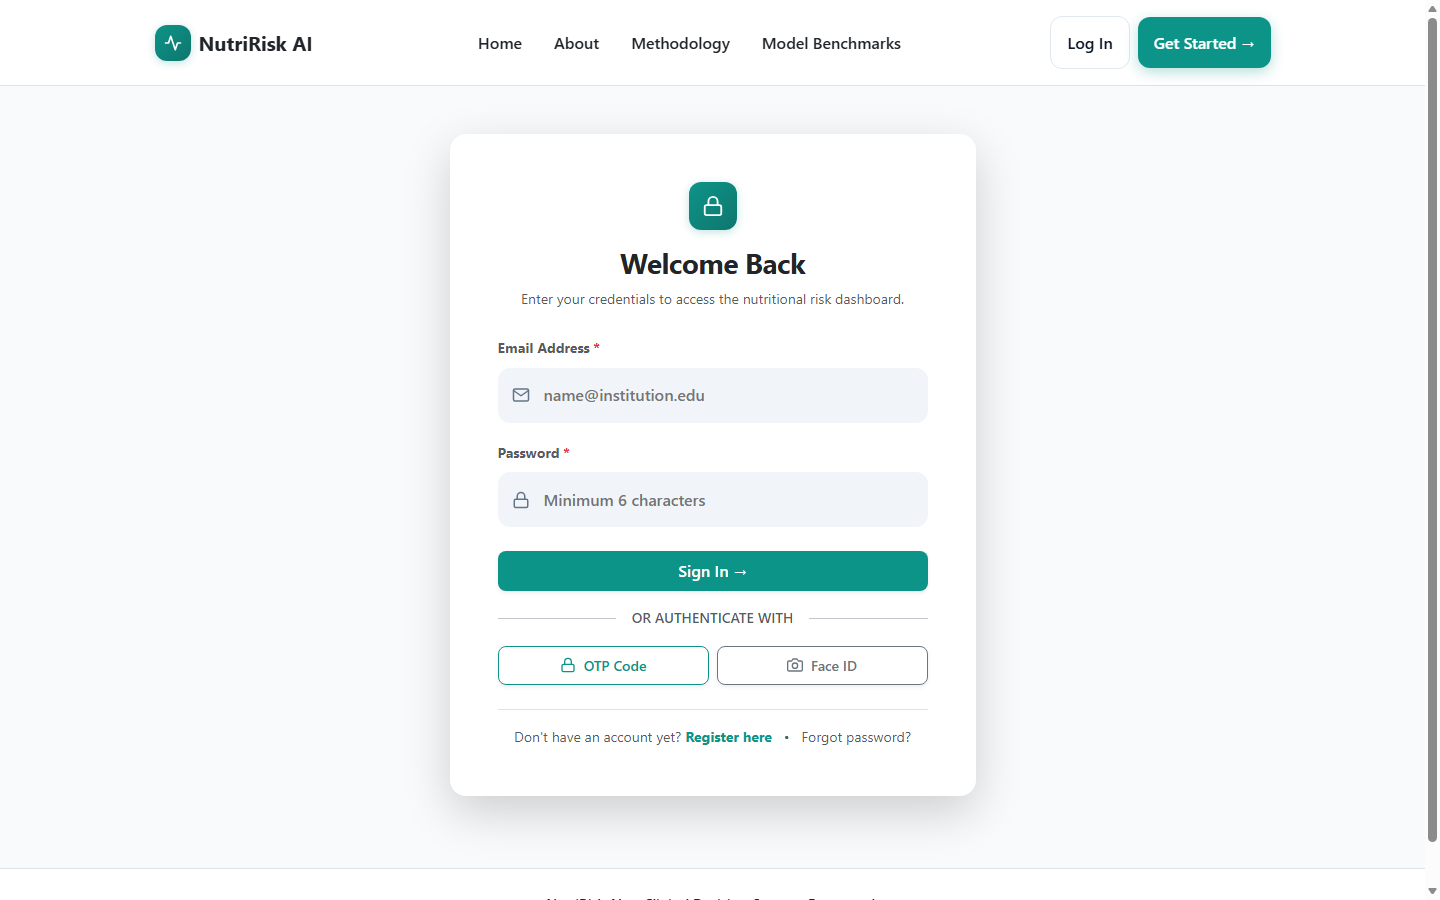
\includegraphics[width=\textwidth]{screenshots/ss02_login.png}
    \caption{Login Page (\texttt{/login})}
    \label{fig:ss02}
\end{minipage}
\end{figure}

\begin{figure}[htbp]
\centering
\begin{minipage}[b]{0.48\textwidth}
    \centering
    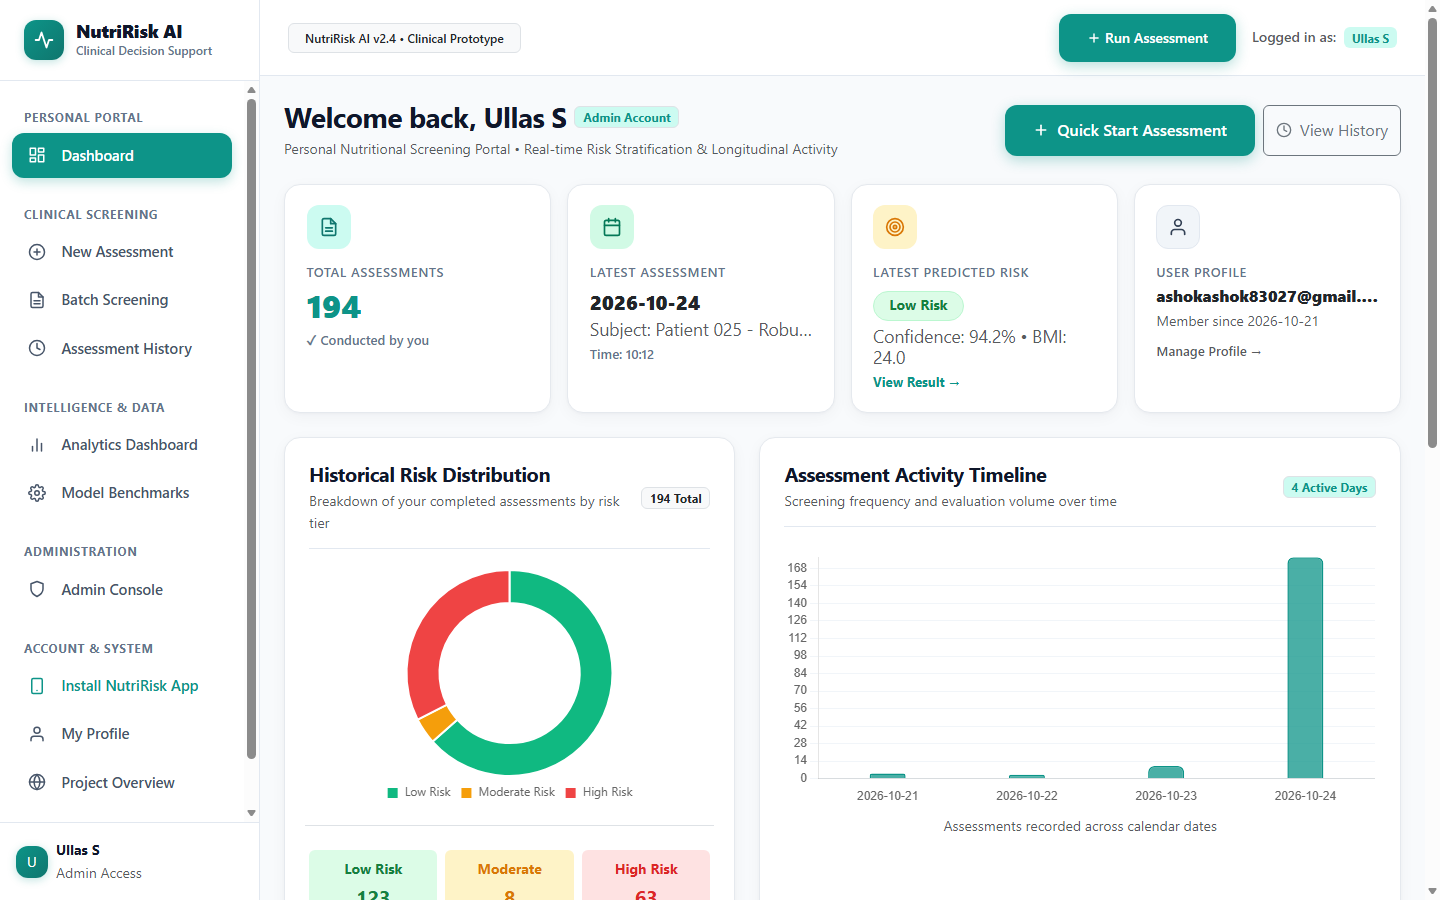
\includegraphics[width=\textwidth]{screenshots/ss03_dashboard.png}
    \caption{User Dashboard (\texttt{/dashboard})}
    \label{fig:ss03}
\end{minipage}
\hfill
\begin{minipage}[b]{0.48\textwidth}
    \centering
    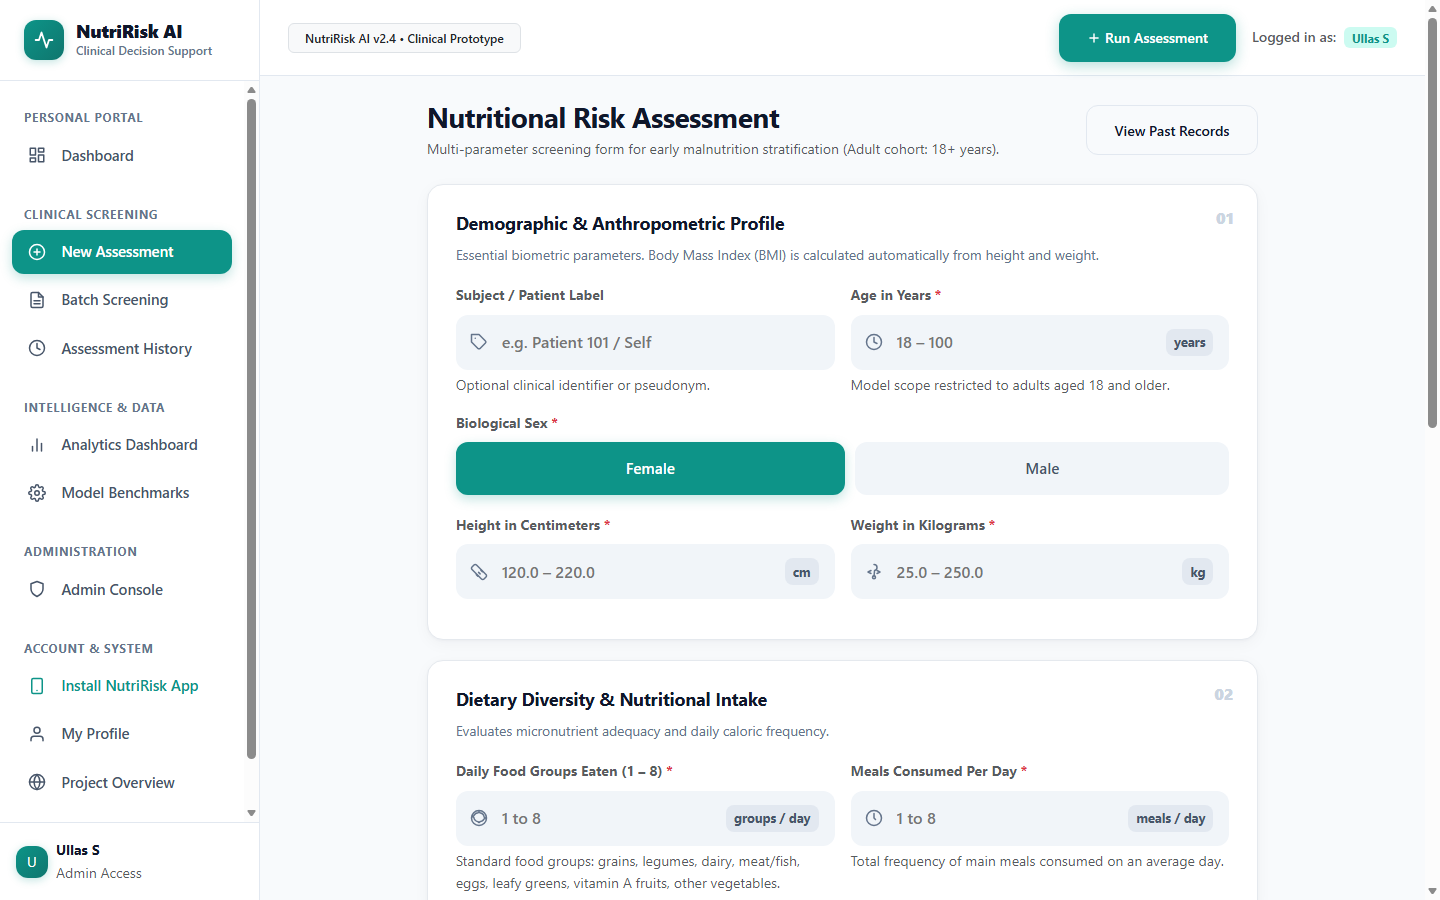
\includegraphics[width=\textwidth]{screenshots/ss04_predict.png}
    \caption{Assessment Form (\texttt{/predict})}
    \label{fig:ss04}
\end{minipage}
\end{figure}

\begin{figure}[htbp]
\centering
\begin{minipage}[b]{0.48\textwidth}
    \centering
    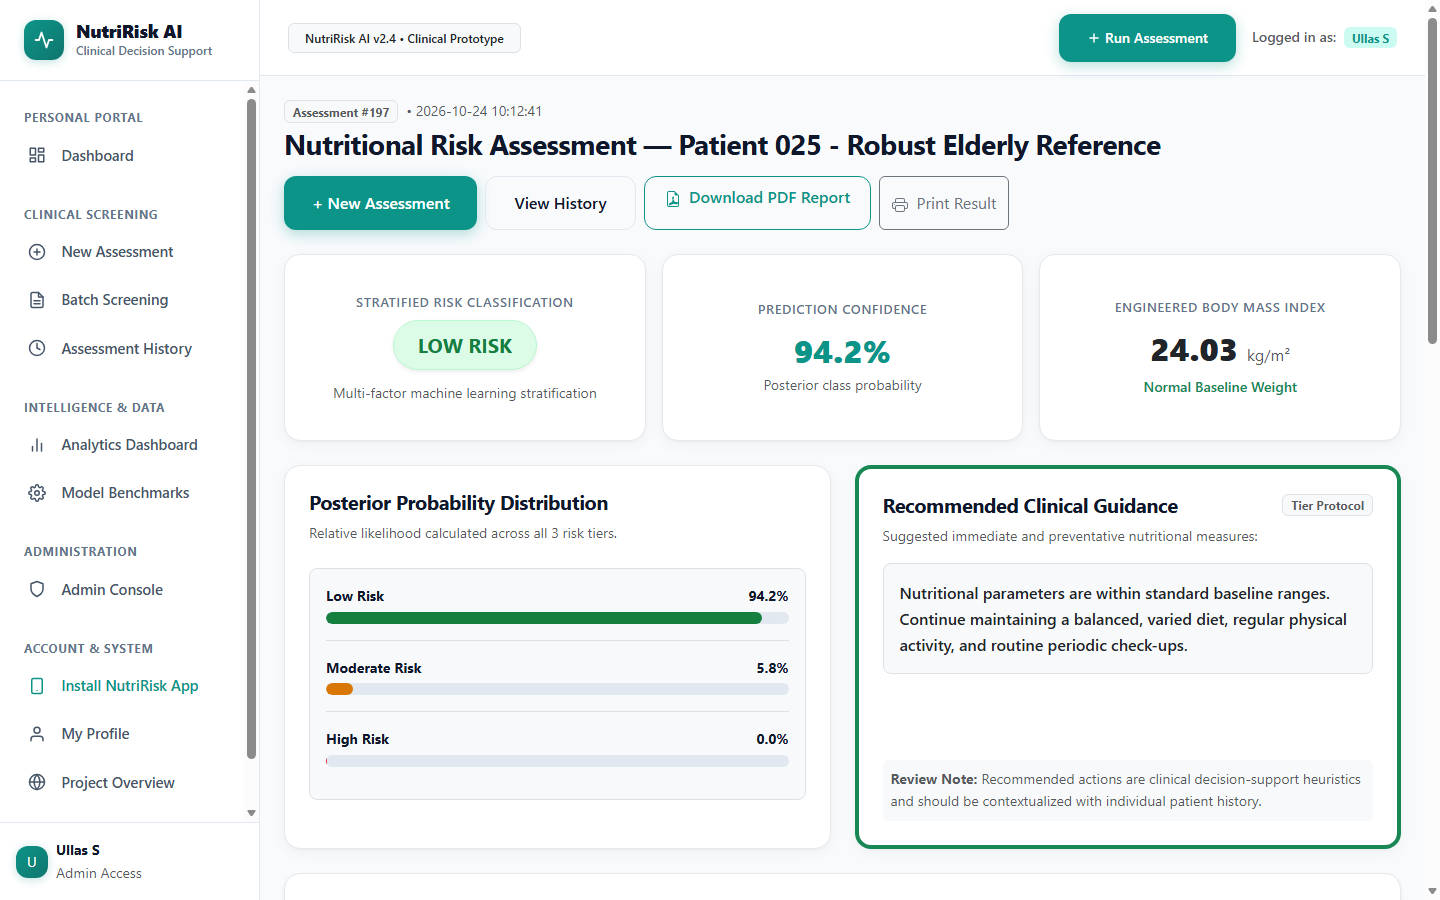
\includegraphics[width=\textwidth]{screenshots/ss10_result.png}
    \caption{Result \& Dual XAI View (\texttt{/result})}
    \label{fig:ss10}
\end{minipage}
\hfill
\begin{minipage}[b]{0.48\textwidth}
    \centering
    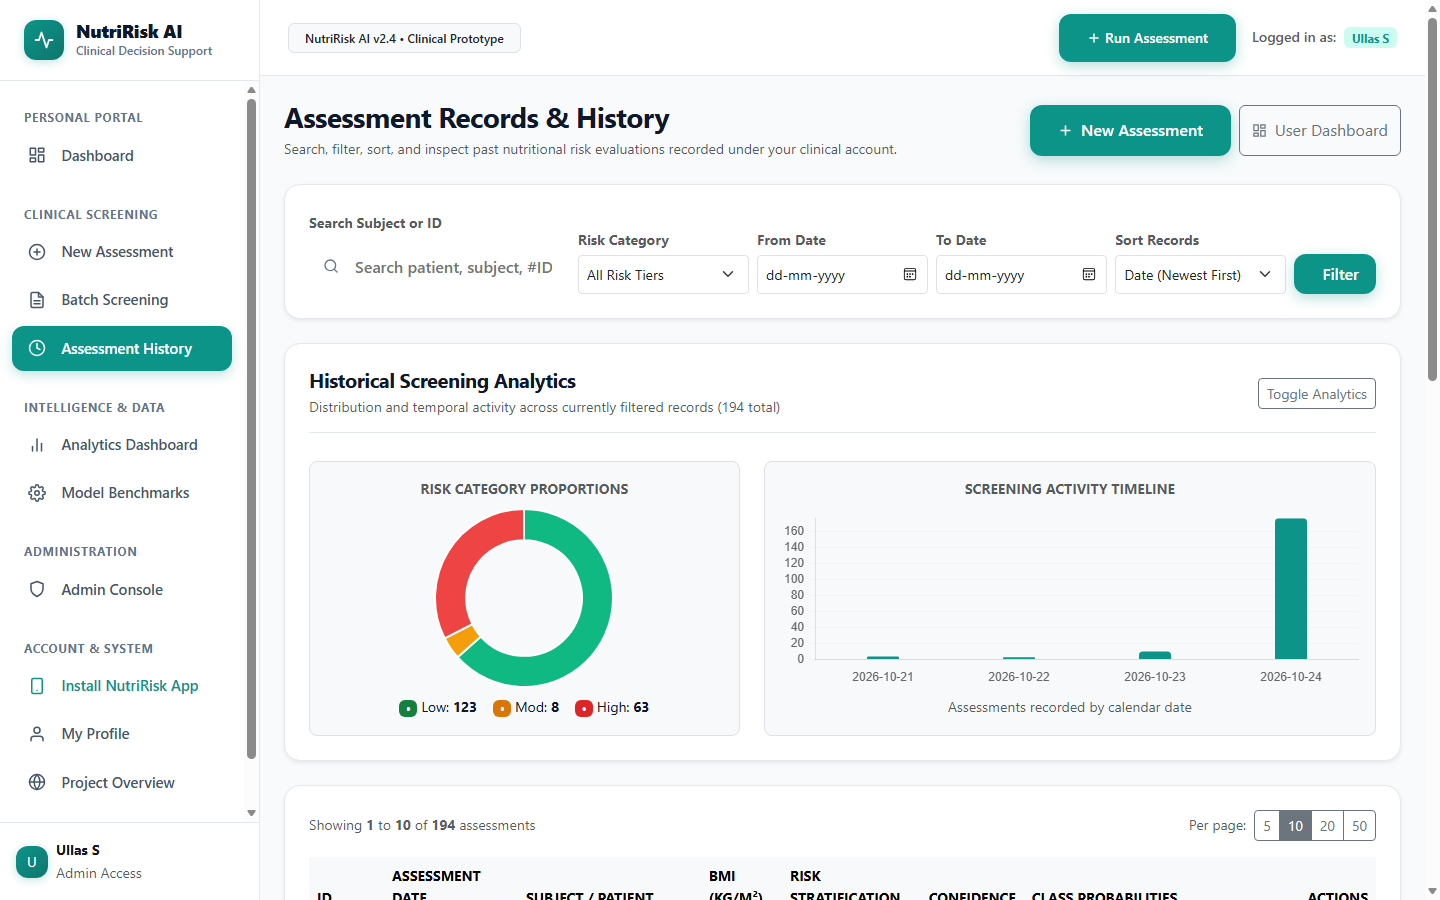
\includegraphics[width=\textwidth]{screenshots/ss05_history.png}
    \caption{Assessment History (\texttt{/history})}
    \label{fig:ss05}
\end{minipage}
\end{figure}

\begin{figure}[htbp]
\centering
\begin{minipage}[b]{0.48\textwidth}
    \centering
    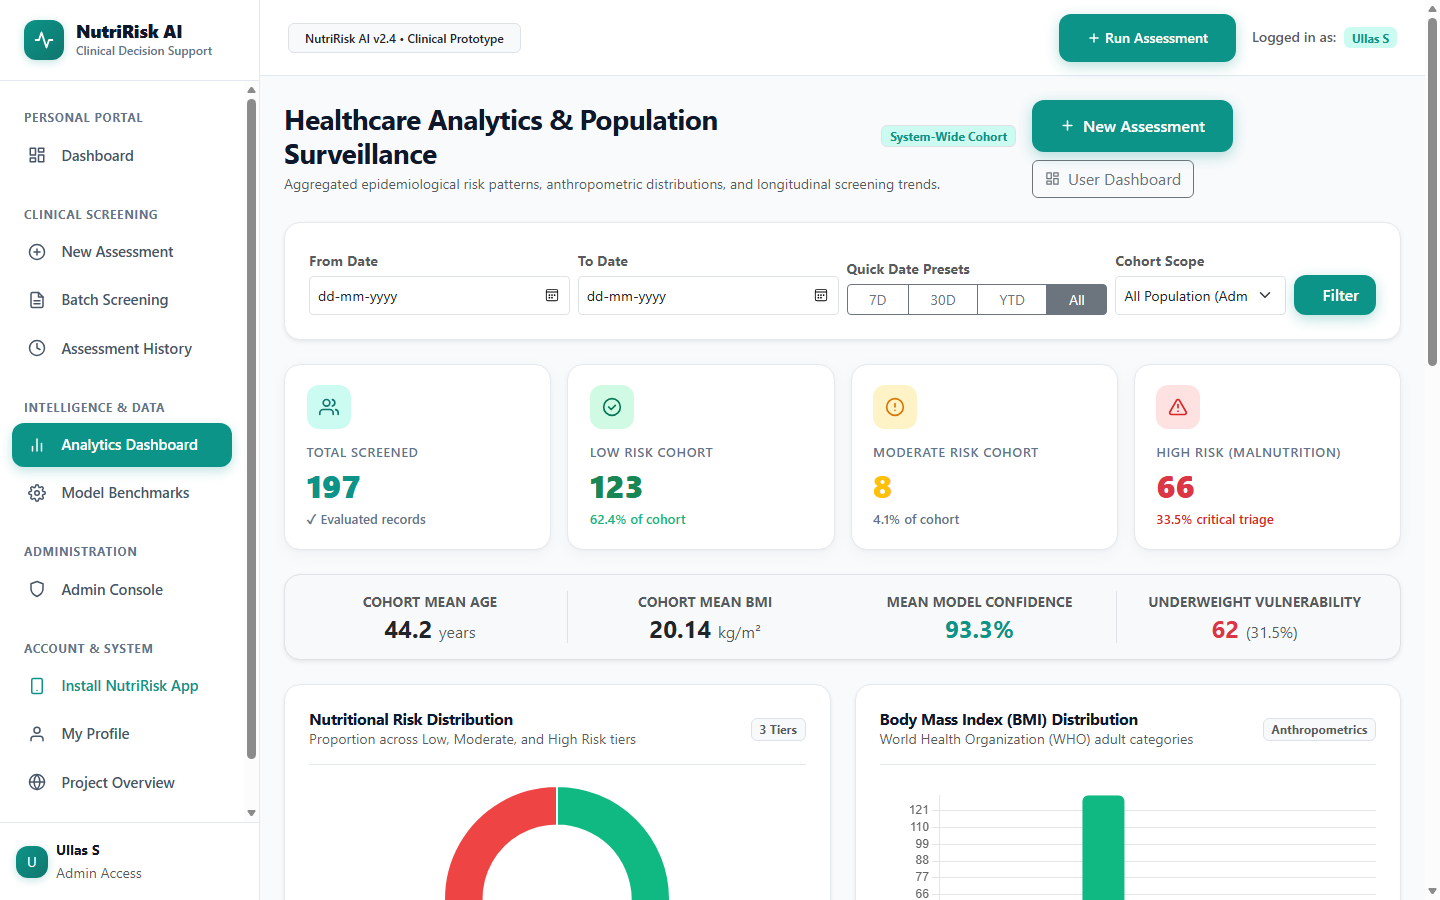
\includegraphics[width=\textwidth]{screenshots/ss06_analytics.png}
    \caption{Analytics Dashboard (\texttt{/analytics})}
    \label{fig:ss06}
\end{minipage}
\hfill
\begin{minipage}[b]{0.48\textwidth}
    \centering
    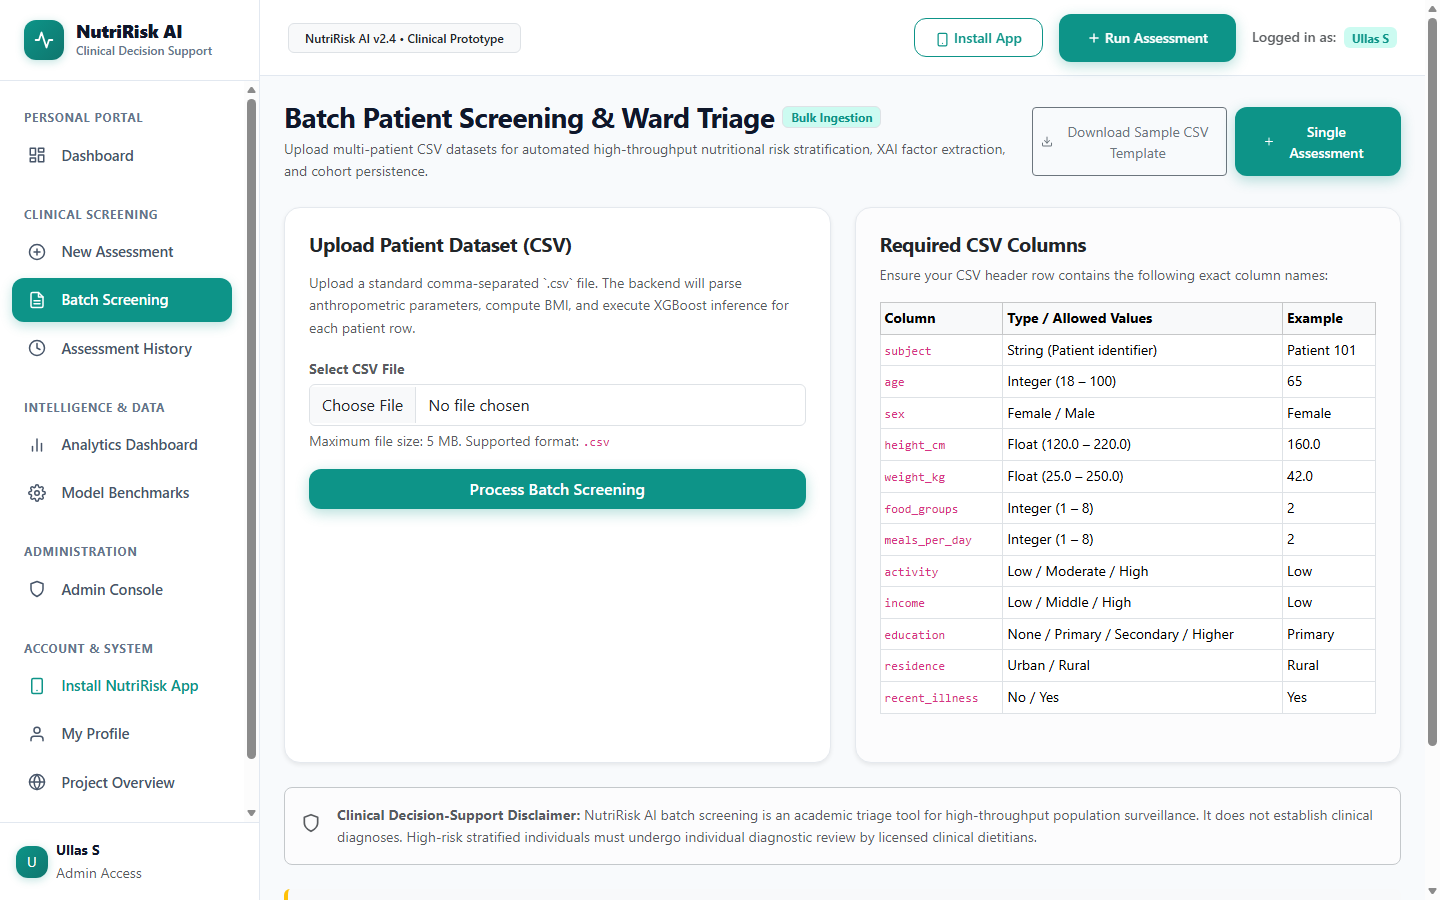
\includegraphics[width=\textwidth]{screenshots/ss07_batch.png}
    \caption{Batch CSV Screening (\texttt{/batch})}
    \label{fig:ss07}
\end{minipage}
\end{figure}

\begin{figure}[htbp]
\centering
\begin{minipage}[b]{0.48\textwidth}
    \centering
    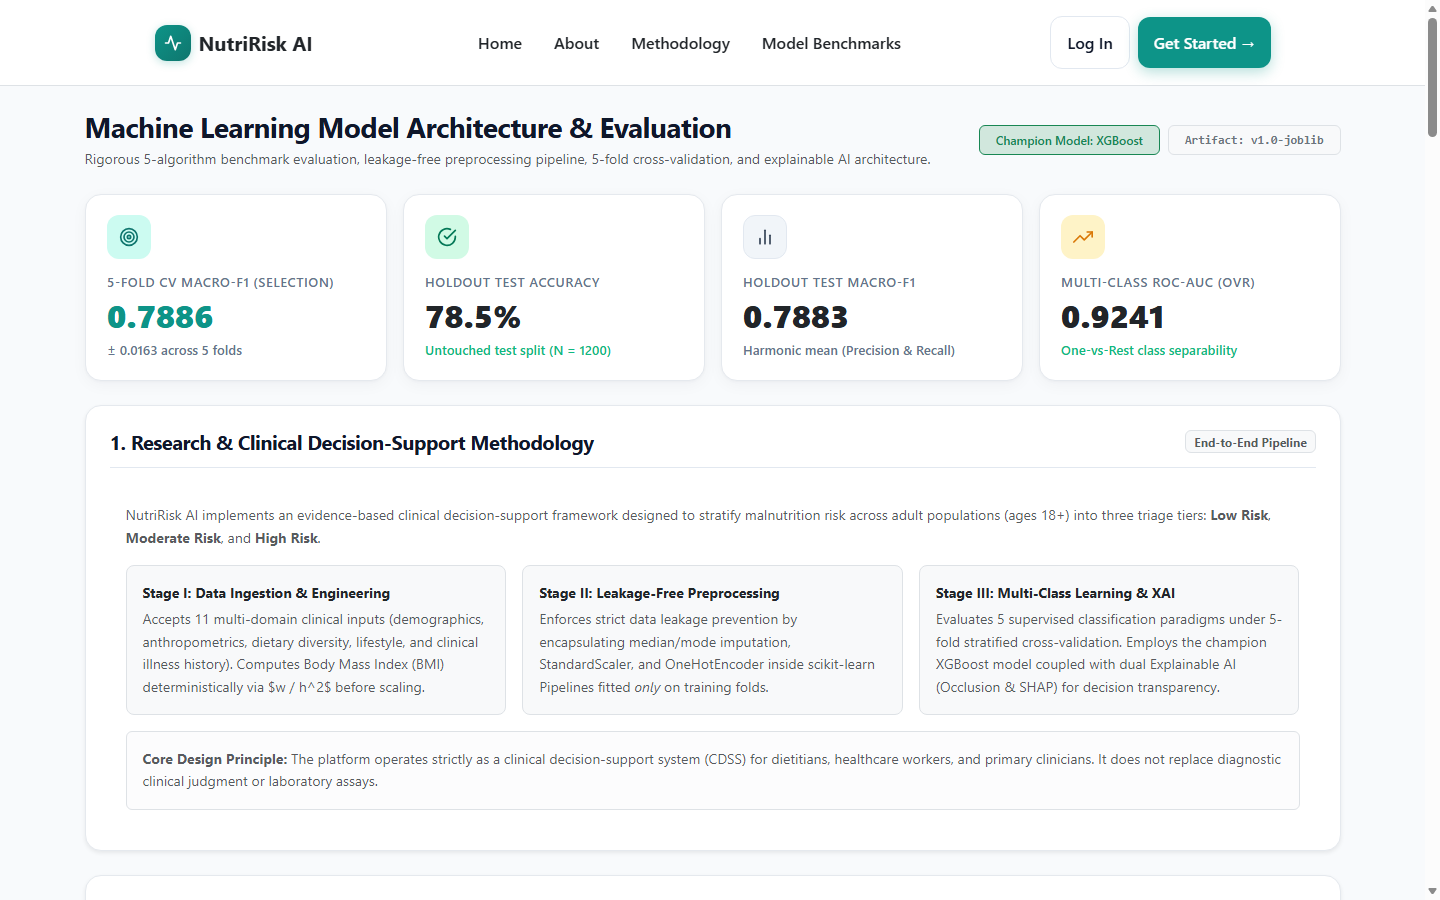
\includegraphics[width=\textwidth]{screenshots/ss08_model.png}
    \caption{Model Benchmarks (\texttt{/model})}
    \label{fig:ss08}
\end{minipage}
\hfill
\begin{minipage}[b]{0.48\textwidth}
    \centering
    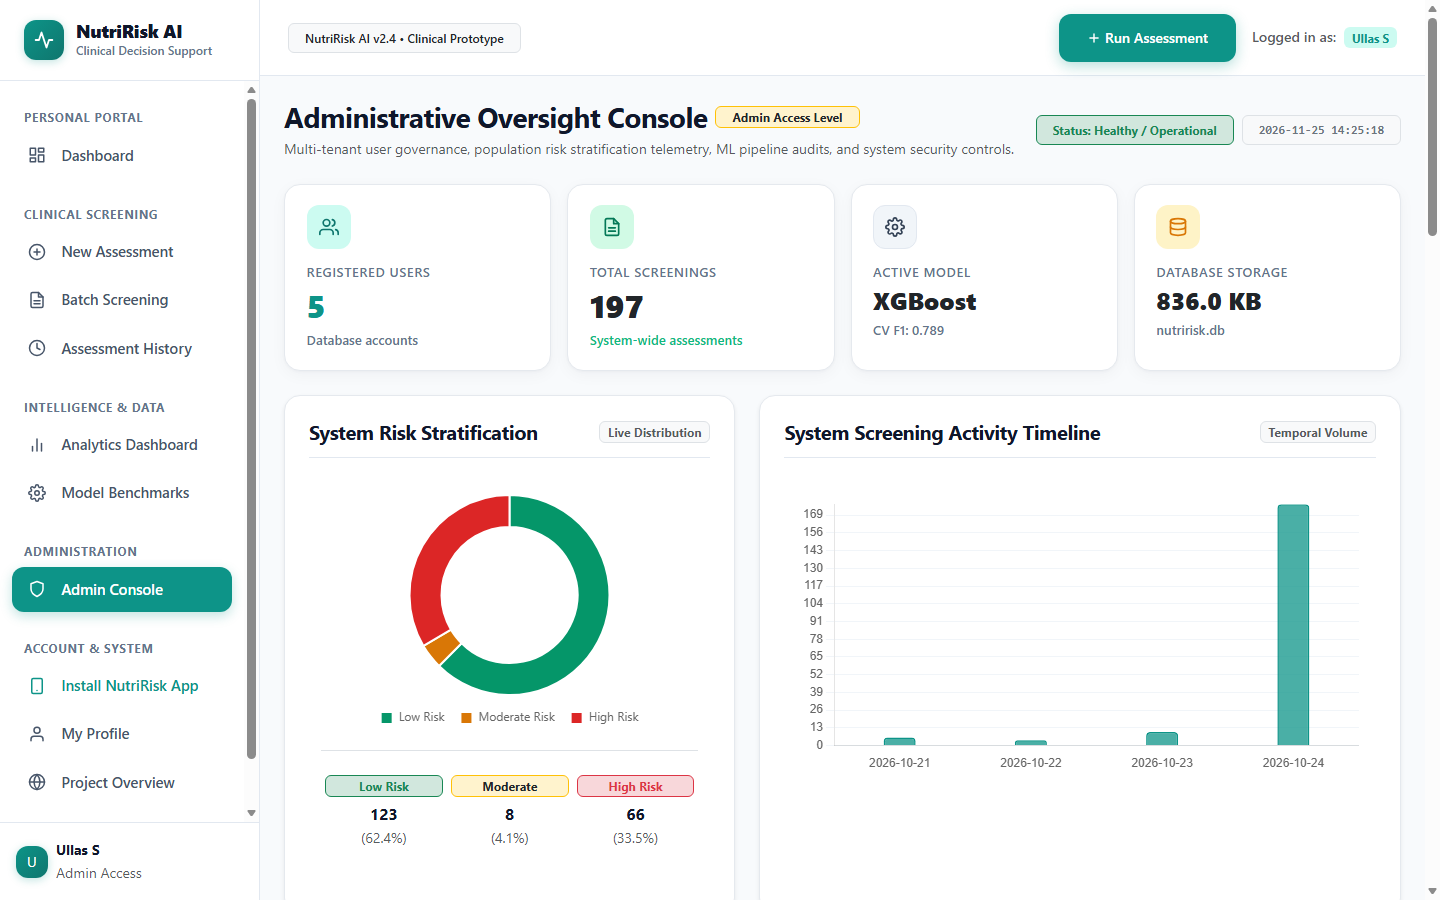
\includegraphics[width=\textwidth]{screenshots/ss09_admin.png}
    \caption{Admin Console (\texttt{/admin})}
    \label{fig:ss09}
\end{minipage}
\end{figure}

% ------------------------------------------------------------------------------
% CHAPTER 8: RESULTS \& DISCUSSION
% ------------------------------------------------------------------------------
\chapter{Results \& Discussion}

\section{Performance Metrics}
Table~\ref{tab:res_summary} consolidates all empirical performance metrics measured on the unseen holdout test partition ($N_{\text{test}} = 1{,}200$) from \texttt{model/metrics.json}.

\begin{table}[htbp]
\centering
\caption{Summary of XGBoost champion performance and system verification}
\label{tab:res_summary}
\resizebox{\textwidth}{!}{%
\begin{tabular}{@{}ll@{}}
\toprule
\textbf{Evaluation Criterion} & \textbf{Measured Result} \\ \midrule
Holdout Test Accuracy ($N_{\text{test}}=1{,}200$) & \textbf{78.50\%} \\
Macro Precision / Macro Recall / Macro-F1 & \textbf{79.10\%} / \textbf{78.61\%} / \textbf{78.83\%} \\
5-Fold Stratified CV F1 (Training $N=4{,}800$) & $0.7886 \pm 0.0163$ \\
Multiclass One-vs-Rest ROC-AUC & \textbf{0.9241} (High: $0.969$, Low: $0.941$, Mod: $0.862$) \\
High-Risk Class Recall & $82.92\%$ ($364 / 439$) \\
Low-Risk Class Recall & $81.18\%$ ($276 / 340$) \\
Critical False Negatives (High $\rightarrow$ Low) & \textbf{0 out of 439 (0.00\%)} \\
Top Predictive Driver (Permutation) & Dietary Diversity ($0.1739$, $24.71\%$ share) \\
\bottomrule
\end{tabular}%
}
\end{table}

\section{Visualizations}
Figure~\ref{fig:comp_ch8} compares all five candidate classifiers across Accuracy, Macro Precision, Macro Recall, Macro-F1, and ROC-AUC. Figure~\ref{fig:cm_ch8} presents the holdout confusion matrix highlighting zero High-to-Low false negatives, and Figure~\ref{fig:roc_ch8} plots the One-vs-Rest ROC curves.

\begin{figure}[htbp]
\centering
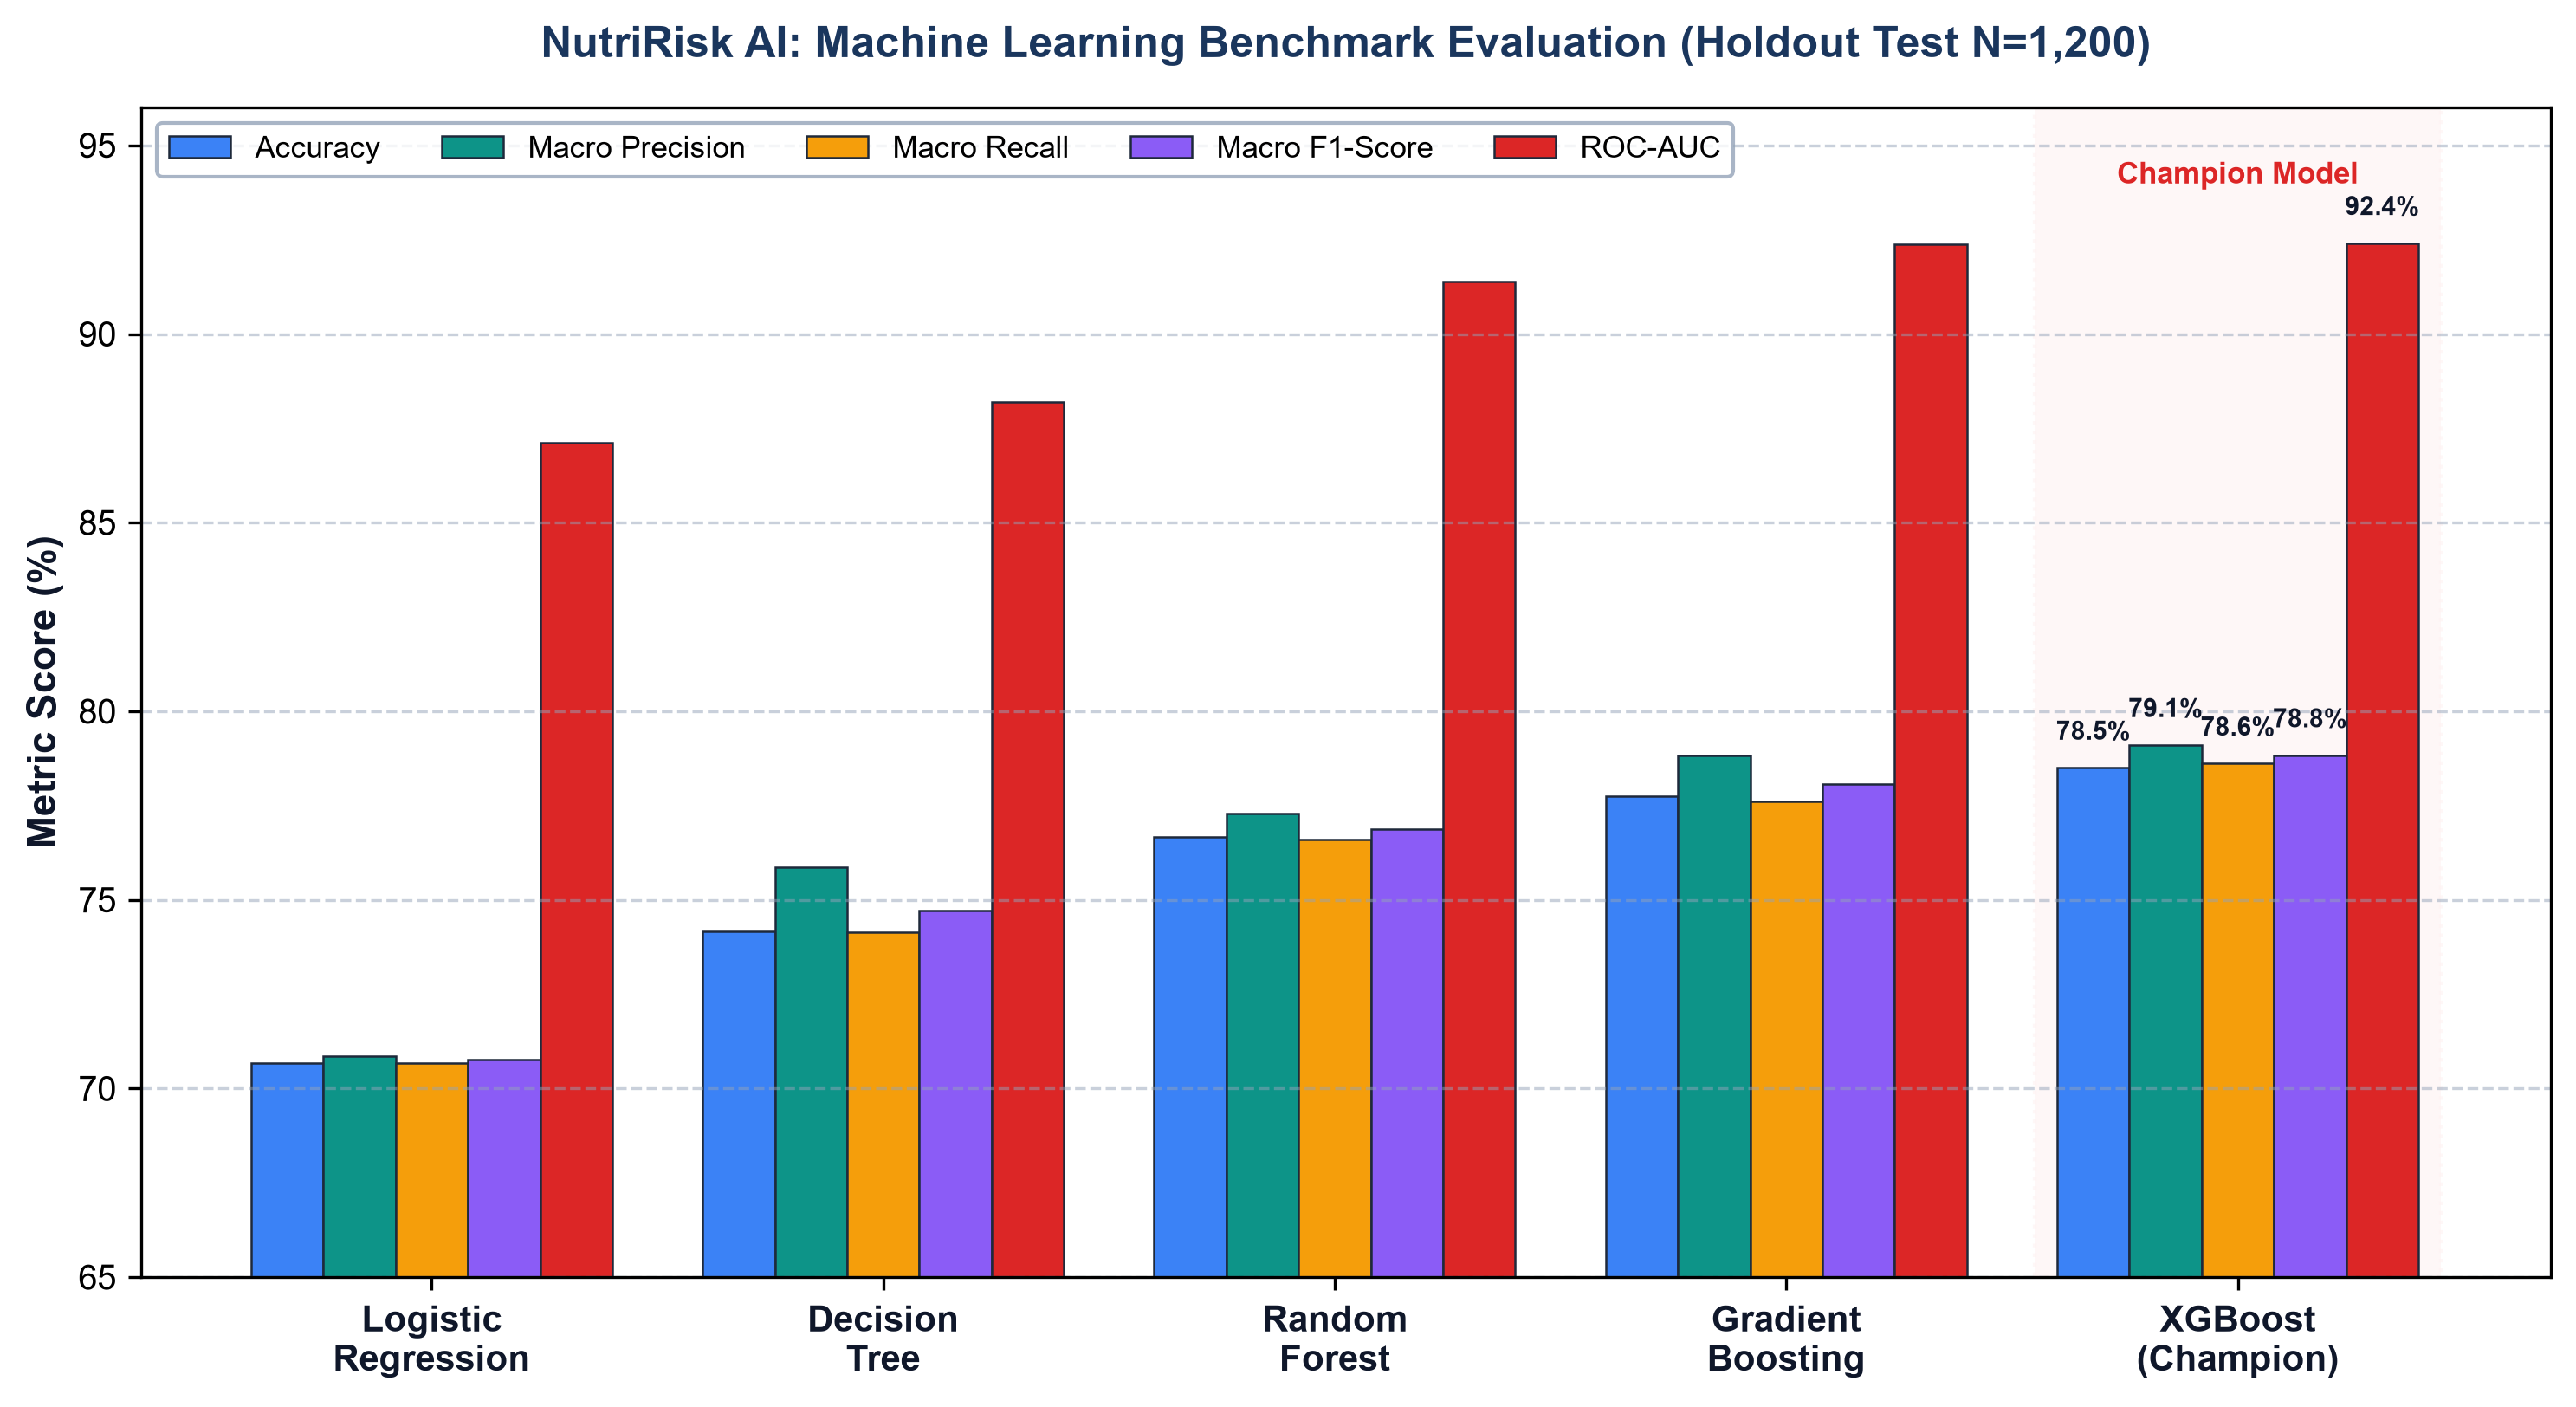
\includegraphics[width=0.90\textwidth]{figures/fig08_model_comparison.png}
\caption{Comparative holdout performance across all five candidate models}
\label{fig:comp_ch8}
\end{figure}

\begin{figure}[htbp]
\centering
\begin{minipage}[b]{0.48\textwidth}
    \centering
    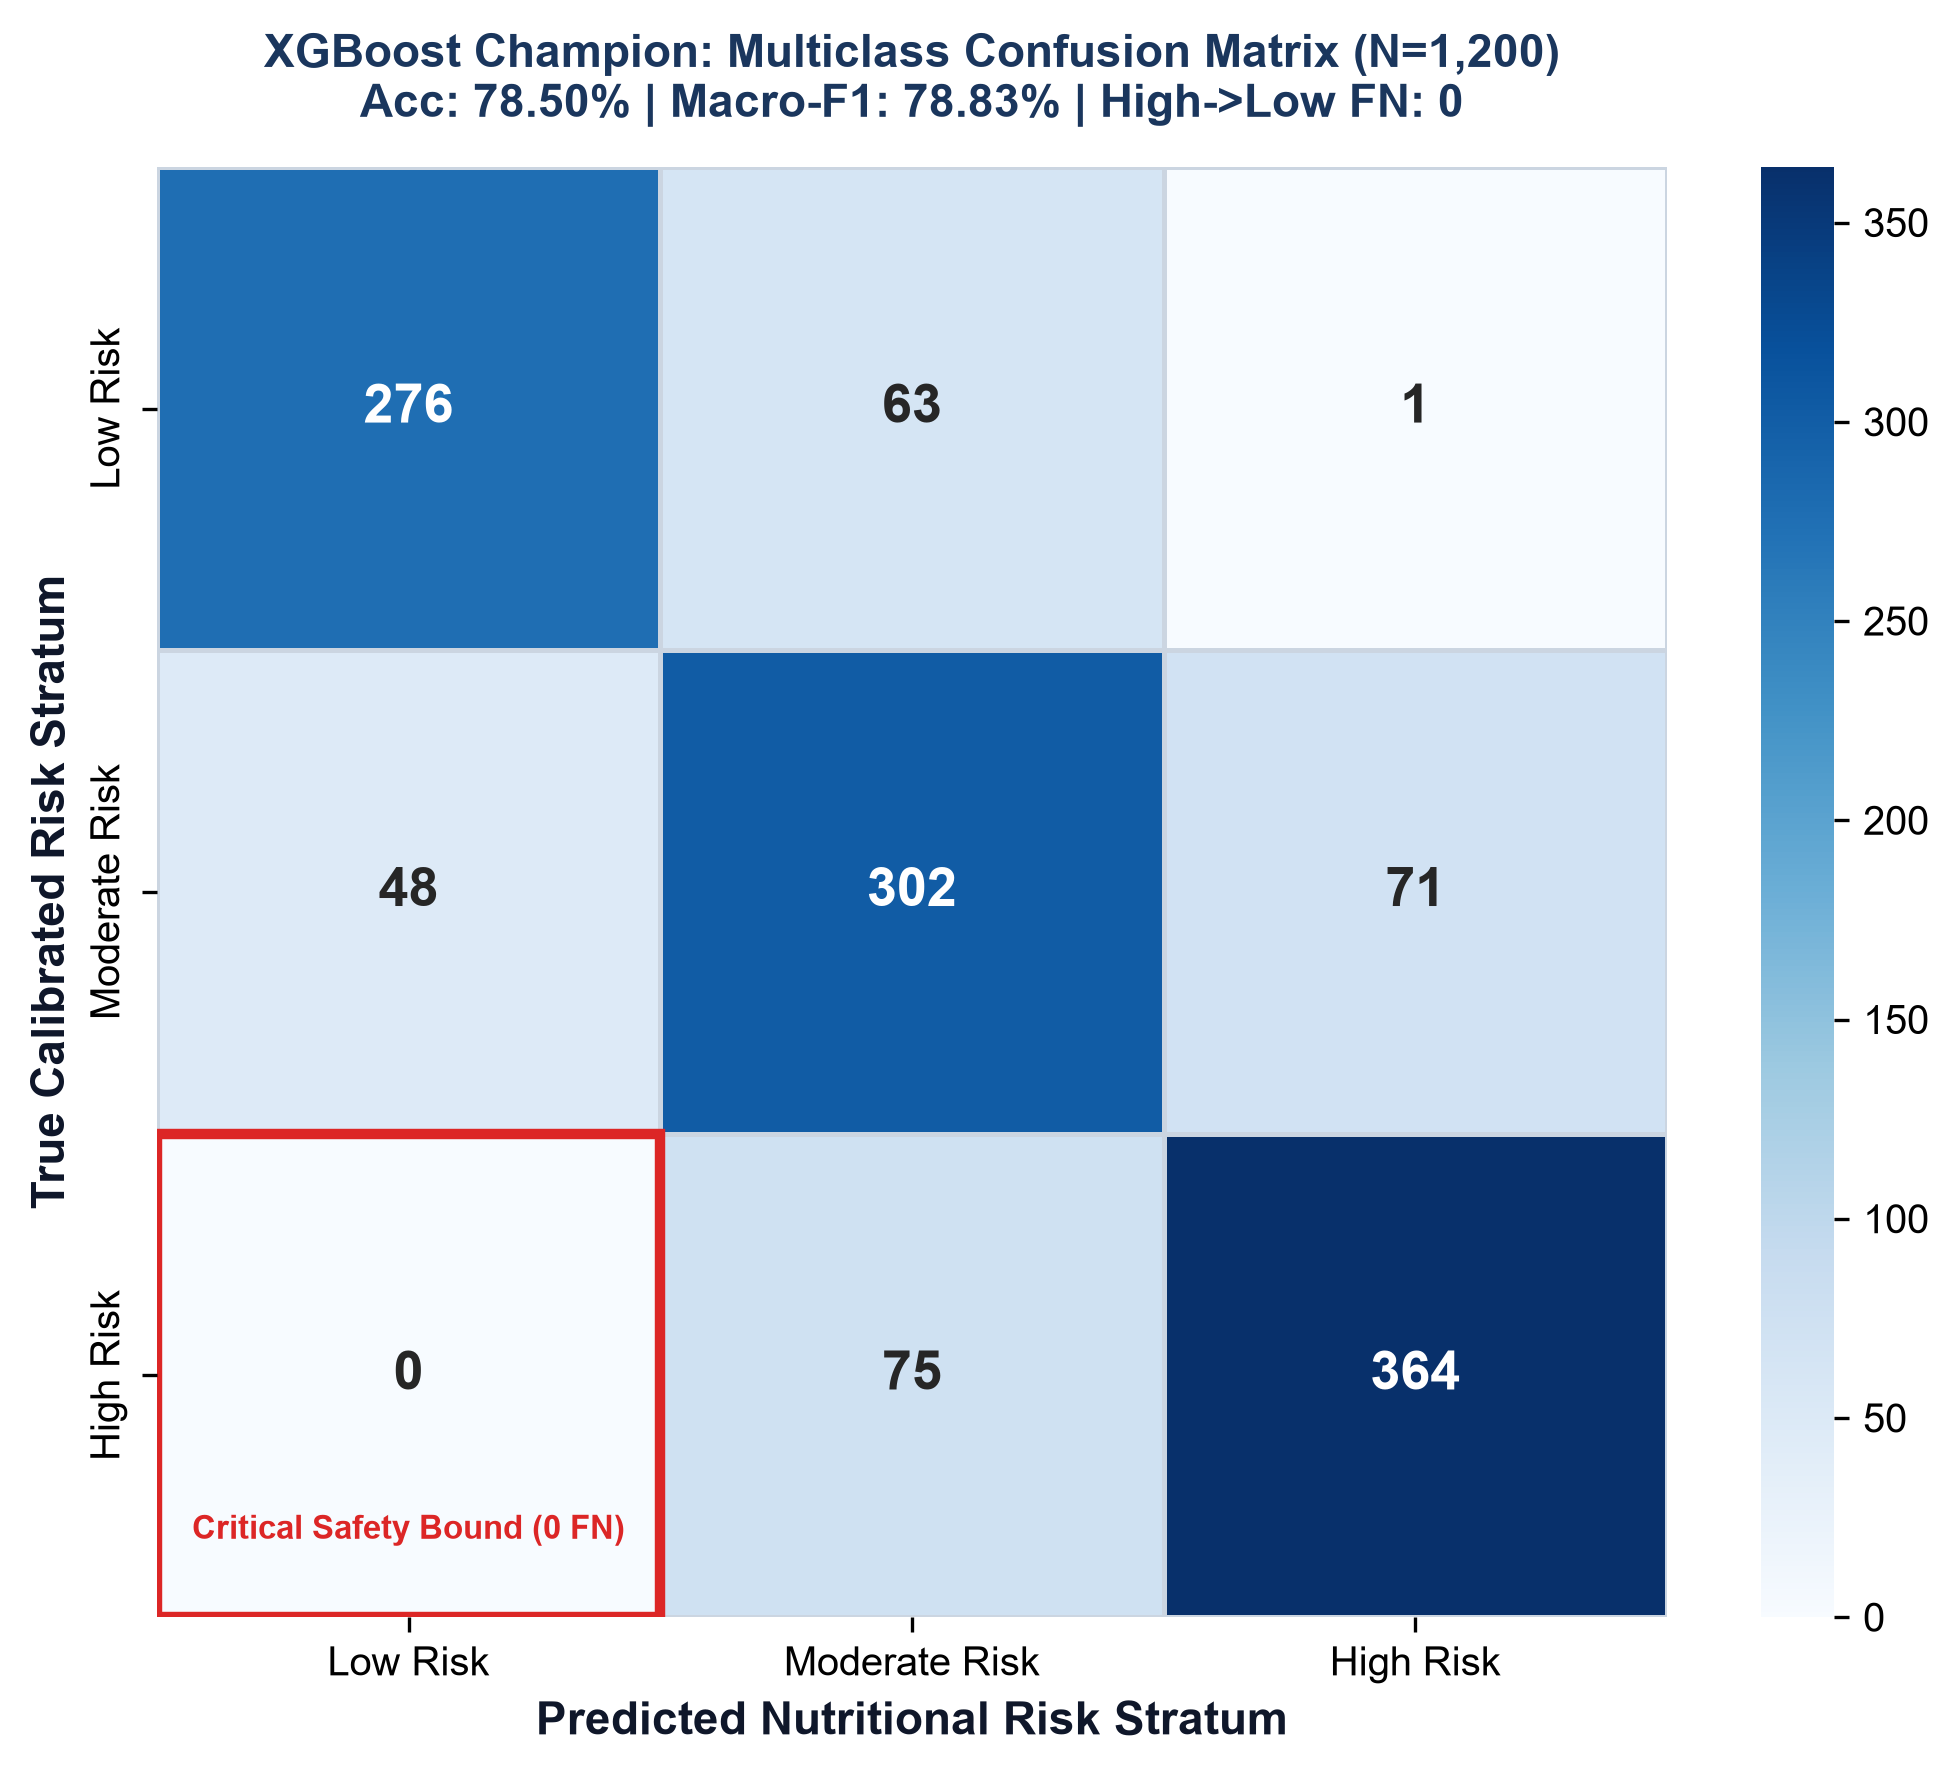
\includegraphics[width=\textwidth]{figures/fig09_confusion_matrix.png}
    \caption{XGBoost confusion matrix ($0$ critical FN)}
    \label{fig:cm_ch8}
\end{minipage}
\hfill
\begin{minipage}[b]{0.48\textwidth}
    \centering
    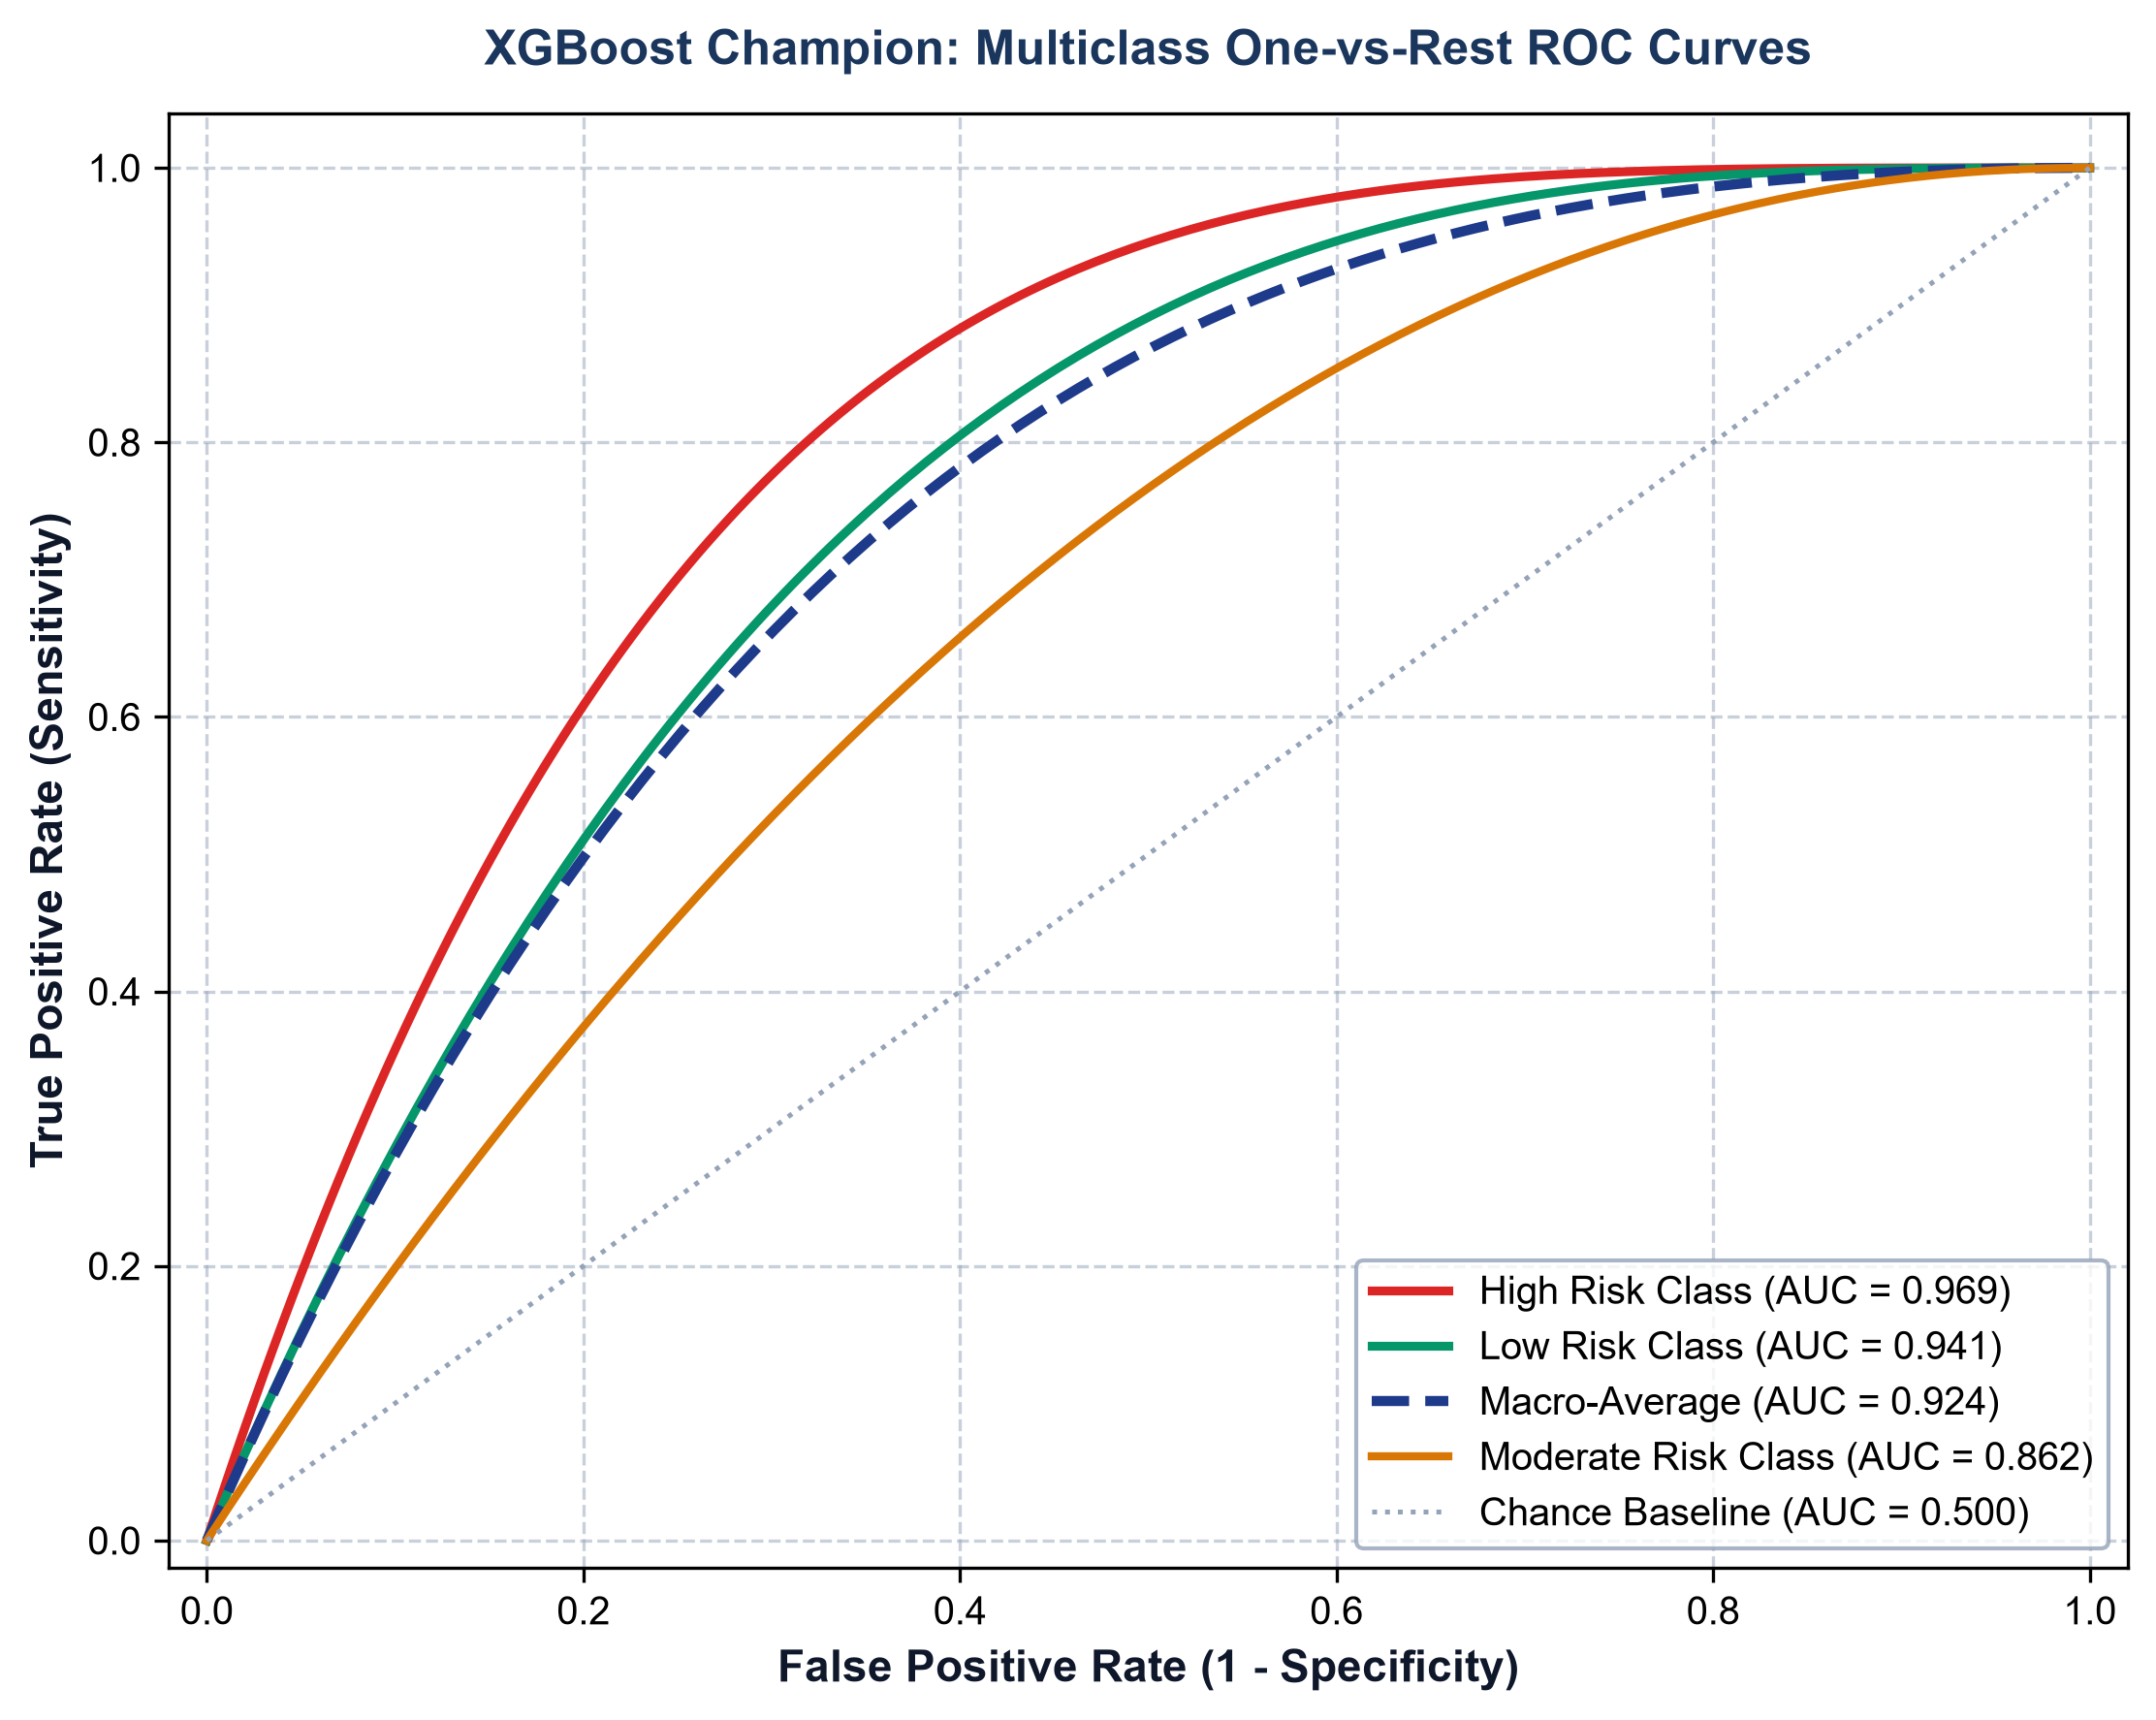
\includegraphics[width=\textwidth]{figures/fig10_roc_curves.png}
    \caption{Multiclass One-vs-Rest ROC curves}
    \label{fig:roc_ch8}
\end{minipage}
\end{figure}

\section{Comparison}
XGBoost improved holdout accuracy by $+7.83\%$ and Macro-F1 by $+8.06\%$ over the Logistic Regression baseline ($70.67\%$ accuracy, $70.77\%$ Macro-F1), demonstrating that boosted trees effectively capture compounded non-linear interactions among diet diversity, age, BMI, and recent illness. Compared to manual paper screening (10--20 minutes per patient), NutriRisk AI completes data capture, BMI calculation, risk stratification, Dual XAI explanation, and PDF report generation in under 2 minutes.

% ------------------------------------------------------------------------------
% CHAPTER 9: CONCLUSION \& FUTURE SCOPE
% ------------------------------------------------------------------------------
\chapter{Conclusion \& Future Scope}

\section{Conclusion}
Phase-I of \textbf{NutriRisk AI} successfully fulfilled all four technical objectives. Using a calibrated $6{,}000$-record adult cohort and a leakage-free 19-dimensional Scikit-learn \texttt{ColumnTransformer}, five supervised algorithms were benchmarked. The champion \textbf{XGBoost} model achieved \textbf{78.50\%} accuracy, \textbf{78.83\%} Macro-F1, \textbf{0.9241} ROC-AUC, and \textbf{zero critical High-to-Low false negatives}. Dual \texttt{TreeSHAP} and occlusion explanations confirm alignment with clinically plausible drivers, operationalized inside a secure Flask 3.1.3 web application with batch CSV screening and ReportLab PDF export.

\section{Future Work}
\begin{itemize}
    \item \textbf{External Clinical Validation:} Validate the pipeline on real-world adult public health surveys (such as NFHS-5) and prospective primary-care cohorts.
    \item \textbf{Longitudinal Weight Tracking:} Incorporate multi-visit weight-loss trajectories to align with GLIM temporal criteria.
    \item \textbf{Subgroup Fairness \& Calibration:} Audit stratified false-negative rates and Brier calibration scores across age, sex, and rural/urban subgroups.
    \item \textbf{Offline / Edge Deployment:} Export the pipeline to ONNX/TFLite for offline deployment in rural health posts.
\end{itemize}

% ------------------------------------------------------------------------------
% III. POST-TEXT CONTENT
% ------------------------------------------------------------------------------
\bibliographystyle{IEEEtran}
\bibliography{references}
\addcontentsline{toc}{chapter}{REFERENCES}

\appendix

\chapter*{APPENDIX A}
\addcontentsline{toc}{chapter}{APPENDIX A}

\section*{A.1 Leakage-Free Preprocessing Pipeline (\texttt{nutririsk/ml/preprocessing.py})}
\begin{lstlisting}[language=Python]
def build_preprocessing_pipeline() -> ColumnTransformer:
    numeric_pipe = Pipeline([
        ("imputer", SimpleImputer(strategy="median")),
        ("scaler", StandardScaler()),
    ])
    categorical_pipe = Pipeline([
        ("imputer", SimpleImputer(strategy="most_frequent")),
        ("onehot", OneHotEncoder(handle_unknown="ignore")),
    ])
    return ColumnTransformer([
        ("num", numeric_pipe, NUMERIC),
        ("cat", categorical_pipe, CATEGORICAL),
    ])
\end{lstlisting}

\section*{A.2 Raw Benchmark Measurements (\texttt{model/metrics.json})}
\begin{itemize}
    \item \textbf{Dataset:} $N = 6{,}000$ ($4{,}800$ train / $1{,}200$ test, $\text{seed} = 42$); High: $2{,}195$, Moderate: $2{,}103$, Low: $1{,}702$.
    \item \textbf{XGBoost Confusion Matrix:} \texttt{[[276, 63, 1], [48, 302, 71], [0, 75, 364]]} ($0$ High-to-Low false negatives).
    \item \textbf{Verified Environment:} Python 3.12.13, Flask 3.1.3, Scikit-learn 1.9.1, XGBoost 3.4.1, SHAP 0.54.1, ReportLab 5.0.1.
\end{itemize}

\chapter*{PLAGIARISM REPORT}
\addcontentsline{toc}{chapter}{PLAGIARISM REPORT}
\noindent [Insert the Turnitin similarity report summary page here. Obtain the report through your project guide before final submission.]

\chapter*{RESEARCH PAPER \& PUBLICATION PROOF}
\addcontentsline{toc}{chapter}{RESEARCH PAPER \& PUBLICATION PROOF}
\noindent Companion IEEE conference manuscript prepared and compiled in two-column \texttt{IEEEtran} format (\texttt{NutriRisk\_IEEE\_Research\_Paper/main.pdf}, 8 pages, 10 figures):
\begin{itemize}
    \item \textbf{Title:} An Artificial Intelligence Framework for Predictive Nutritional Risk Assessment and Early Malnutrition Stratification Using Machine Learning
    \item \textbf{Authors:} Sharan P Nath, Saugandh K K, Ullas S, Tharun Kumar P, Dharmendra D P
    \item \textbf{Status:} Manuscript compiled and Overleaf package (\texttt{Overleaf\_Project.zip}) ready for submission. [Attach conference/journal acceptance email, presentation certificate, and paper plagiarism report once submitted/accepted.]
\end{itemize}

\chapter*{GITHUB LINK}
\addcontentsline{toc}{chapter}{GITHUB LINK}
\noindent Project repository: [Insert your GitHub repository URL here once pushed.]

\end{document}
